\documentclass[12pt]{article}
\usepackage[T1]{fontenc}
\usepackage[utf8]{inputenc}
\usepackage{amsmath,amssymb,amsthm,mathtools,bm}
\usepackage{newtxtext,newtxmath}
\usepackage{microtype}
\usepackage{booktabs,array,threeparttable,graphicx,float}
\usepackage[font=small,labelfont=bf]{caption}
\usepackage[margin=1in]{geometry}
\usepackage{setspace}
\usepackage[round,authoryear]{natbib}
\usepackage{xurl}
\usepackage{xr-hyper}
\usepackage[hidelinks]{hyperref}
\usepackage{enumitem}
\usepackage{ragged2e}

\ifdefined\pdfminorversion
  \pdfminorversion=7
\fi

\doublespacing
\setlength{\emergencystretch}{3em}
\setlength{\textfloatsep}{12pt plus 2pt minus 2pt}
\setlength{\floatsep}{10pt plus 2pt minus 2pt}
\setlength{\intextsep}{10pt plus 2pt minus 2pt}

\newtheorem{theorem}{Theorem}
\newtheorem{proposition}{Proposition}
\newtheorem{corollary}{Corollary}
\newtheorem{lemma}{Lemma}
\theoremstyle{definition}
\newtheorem{assumption}{Condition}
\newtheorem{highlevelassumption}{Assumption}
\theoremstyle{remark}
\newtheorem{remark}{Remark}

\newcommand{\E}{\mathbb E}
\newcommand{\Pp}{\mathbb P}
\newcommand{\Var}{\operatorname{Var}}
\newcommand{\Cov}{\operatorname{Cov}}
\newcommand{\Prj}{\Pi_{[0,1]}}
\newcommand{\Ycal}{\mathcal Y}
\newcommand{\Fhat}{\widehat F}
\newcommand{\Ghat}{\widehat G}
\newcommand{\Hhat}{\widehat H}
\newcommand{\lhat}{\widehat\lambda}
\newcommand{\lstar}{\lambda^\star}
\newcommand{\op}{o_{\Pp}}
\newcommand{\Op}{O_{\Pp}}
\newcommand{\ip}[2]{\langle #1,#2\rangle_{\nu}}
\newcommand{\normnu}[1]{\lVert #1\rVert_{\nu}}
\DeclareMathOperator*{\argmin}{arg\,min}

\newenvironment{procedurebox}
{\begin{center}\begin{minipage}{0.94\textwidth}\hrule\vspace{0.6em}}
{\vspace{0.4em}\hrule\end{minipage}\end{center}}

\externaldocument[][nocite]{../paper/manuscript_blind}
\makeatletter
\@ifundefined{r@eq:observable-G}{}{%
  \expandafter\let\csname r@eq:G-observable\expandafter\endcsname
  \csname r@eq:observable-G\endcsname}
\makeatother
\title{Supplement to ``Surrogate-Assisted Local Conditional Distribution Inference with Scarce Reference Outcomes''}
\author{}
\date{}

\begin{document}
\renewcommand{\thetable}{S\arabic{table}}
\renewcommand{\thefigure}{S\arabic{figure}}
\makeatletter
\renewcommand*\l@subsection{\@dottedtocline{2}{1.5em}{3.1em}}
\makeatother
\maketitle
\begingroup
\small
\tableofcontents
\endgroup
\clearpage

\section{Symbol guide}
\label{sec:supp-symbols}

\begin{center}
\footnotesize
\begin{tabular}{>{\raggedright\arraybackslash}p{3.0cm}>{\raggedright\arraybackslash}p{10.5cm}}
\toprule
Symbol & Definition \\
\midrule
$O=(W,R,RY)$ & Observed data; $W$ includes broadly observed $X,S$, and $Z_y=1(Y\le y)$. \\
$F_0(y\mid x_0)$ & Conditional CDF of the reference outcome at the target point. \\
$F_{h,0}(y\mid x_0)$ & Kernel-regularized target in \eqref{eq:regular-target}. \\
$F_{h,\mathrm{emp}}(y\mid x_0)$ & Full-data empirical localized CDF used for the EPA and VitalDB controlled-sampling benchmarks. \\
$\pi_M(W)$ & Verification probability; $p_M=E\{\pi_M(W)\}$ and $e_M(W)=\pi_M(W)/p_M$. \\
$N_{M,h}=Mp_Mh^d$ & Nominal local-information rate index used in the process normalization. \\
$q_{0,y}(X)$, $m_{0,y}(W)$ & Threshold regressions given $X$ and $W$, respectively. \\
$U_y(a)$ & Augmented threshold signal in \eqref{eq:pseudo}. \\
$\delta_y^a=a_y-m_{0,y}$ & Generic augmentation error; $\Delta_{M,y}$ and $\Delta_y$ are the triangular and limiting oracle-path errors. \\
$D_y=m_y-q_y$ & Candidate surrogate correction, conditional on the fitting sample. \\
$A_y=m_{0,y}-q_y$ & Correction from the candidate anchor to the true threshold regression. \\
$J_{M,h}(\lambda)$ & Augmentation-dependent integrated local variance along $a_{\lambda,y}=q_y+\lambda D_y$. \\
$G_{M,h}$, $H_{M,h}$ & Alignment and curvature terms in the quadratic criterion. \\
$\lambda_h^{\mathrm{or}}$ & Path-oracle coefficient ($M$ implicit); $\widehat\lambda_{h,k}$ is its fold estimate. \\
$\widehat\mu_{h,G,k}$, $\widehat v_{h,k}$ & Selection-fold kernel mean and empirical transfer weight in \eqref{eq:vhat}. \\
$\mathcal J$, $\mathcal G$, $\mathcal H$ & Criterion quantities multiplied by $p_M$ for a common fixed/scarce-reference scale. \\
$\Psi_{M,y}$ & Scaled path-oracle influence process in \eqref{eq:oracle-process}. \\
$\Gamma_p(y,z)$ & Covariance kernel of the limiting local CDF process. \\
$\mathbf S_h$, $L_h$ & Local-linear population Gram matrix and equivalent weight. \\
$\vartheta$ & Finite signed measure used for a scalar projection of the threshold-indexed CDF. \\
$\rho_{M,k}$, $\rho_k$ & Evaluation-fold sample fraction and its positive limit. \\
\bottomrule
\end{tabular}
\end{center}

Bold symbols denote finite vectors or matrices. A superscript ``eff'' denotes a canonical-gradient quantity, a superscript ``or'' denotes a path-oracle estimator with fitted regressions and population borrowing coefficients, and a superscript ``cl'' denotes an independent-cluster process.

\section{Notation and conditions}
\label{sec:supp-assumptions}

This section collects the conditions used in the proofs. Exact efficiency and transfer results use weighted square integrability. Gain estimation and path-oracle equivalence add sample separation and local second moments. The continuum process adds threshold increments and entropy control. Point-target and quantile inference add smoothness in \(x\) and regularity of the inverse-CDF map.

For each \(M\), let
\[
O_{Mi}=(W_i,R_i,R_iY_i),\qquad i=1,\ldots,M,
\]
be independent and identically distributed within row \(M\). Here \(W\)
contains \(X\), \(S\), and any other broadly observed variables. The primary
designs use \(W=(X,S)\), while an additional observed design variable may
enter the verification probability. Write \(Z_y=1(Y\le y)\),
\[
q_{0,y}(X)=E(Z_y\mid X),
\qquad
m_{0,y}(W)=E(Z_y\mid W).
\]
The joint law of \((W,Y)\) is fixed and the verification law may vary with
\(M\). The threshold set \(\mathcal Y=[\underline y,\overline y]\) is compact. Define
\[
K_h(X-x_0)=K\{(X-x_0)/h\},
\qquad
\mu_h=E K_h(X-x_0),
\]
and
\[
F_{h,0}(y\mid x_0)
=
\frac{E\{K_h(X-x_0)Z_y\}}{\mu_h}.
\]
For an augmentation \(a=\{a_y:y\in\mathcal Y\}\),
\[
U_y(a)=a_y(W)+\frac{R}{\pi_M(W)}\{Z_y-a_y(W)\}.
\]

\begin{assumption}[Sampling and verification]
\label{cond:sampling}
Reference sampling satisfies
\[
R\perp Y\mid W.
\]
Define
\[
p_M=E\{\pi_M(W)\},
\qquad
e_M(W)=\pi_M(W)/p_M.
\]
Then \(p_M\to p\in[0,1]\), \(E\{e_M(W)\}=1\), and constants \(0<c_e<C_e<\infty\) satisfy
\[
c_e\le e_M(W)\le C_e
\]
almost surely. The joint local limit of \(e_M\) and the process path is specified in Condition~\ref{cond:covariance}.
\end{assumption}

\begin{assumption}[Local design and kernel]
\label{cond:kernel}
The point \(x_0\) is interior to the support of \(X\). The density \(f_X\) is positive and continuous at \(x_0\). The kernel \(K:\mathbb R^d\to[0,\infty)\) is bounded, symmetric, compactly supported, and of bounded variation, with
\[
0<\kappa_1=\int K(u)\,du<\infty,
\qquad
0<\kappa_2=\int K^2(u)\,du<\infty.
\]
The bandwidth satisfies
\[
h\to0,
\qquad
Mp_Mh^d\to\infty.
\]
\end{assumption}

For a threshold-indexed function \(b\), define
\begin{equation}
\|b\|_{\mathrm{ver}}^2
=
\sup_{y\in\mathcal Y}
\frac{p_Mh^d}{\mu_h^2}
E\left[
K_h^2(X-x_0)
\left\{\frac1{\pi_M(W)}-1\right\}
b_y^2(W)
\right].
\label{eq:local-ver-metric}
\end{equation}

\begin{assumption}[Candidate paths and sample splitting]
\label{cond:candidates}
The sample is partitioned into three folds \(I_1,I_2,I_3\), with
\[
\rho_{M,j}=|I_j|/M\to\rho_j\in(0,1),
\qquad
\rho_1+\rho_2+\rho_3=1.
\]
Regression fitting, weight selection, and CDF evaluation are assigned to different folds and rotate across them. For each evaluation fold \(k\), its threshold regressions and borrowing weight are constructed from the other two folds. With probability tending to one,
\[
\sup_{k,y,x}|\widehat q_{k,y}(x)|
+
\sup_{k,y,w}|\widehat m_{k,y}(w)|
\le B
\]
for a finite constant \(B\).

Write
\[
\varepsilon_M=p_M\varepsilon_{H,M},
\qquad
\mathcal H_{h,k}=p_MH_{M,h,k}.
\]
Here and below, dependence on \(M\) is implicit for fold-specific population criterion quantities. The theoretical stabilizer satisfies \(\varepsilon_{H,M}\downarrow0\). For every evaluation fold, \(\mathcal H_{h,k}\to H_{\infty,k}\in[0,\infty)\). If \(H_{\infty,k}>0\), then
\[
\varepsilon_M=o(H_{\infty,k});
\]
if \(H_{\infty,k}=0\), the fitted correction path satisfies Condition~\ref{cond:path-compatibility}.

Conditional on the fitted regressions, let \(\lambda_{h,k}^{\mathrm{or}}\) minimize their population transfer criterion, with dependence on \(M\) implicit, and set
\[
a_{k,y}^{\mathrm{or}}
=
\widehat q_{k,y}
+
\lambda_{h,k}^{\mathrm{or}}
(\widehat m_{k,y}-\widehat q_{k,y}).
\]
There exist deterministic triangular paths \(q_{M,y}(X)\), \(m_{M,y}(W)\), their population-minimizing coefficient \(\lambda_{M,h}\), and
\[
a_{M,y}
=
q_{M,y}
+
\lambda_{M,h}
(m_{M,y}-q_{M,y})
\]
such that, uniformly over \(k\),
\[
\|a_k^{\mathrm{or}}-a_M\|_{\mathrm{ver}}
=o_{\mathbb P}(1).
\]
There is a bounded deterministic path \(a_\infty=\{a_{\infty,y}:y\in\mathcal Y\}\) such that, for every finite \(C\),
\begin{equation}
\sup_{y\in\mathcal Y}\sup_{\|x-x_0\|\le Ch}
E\{(a_{M,y}-a_{\infty,y})^2\mid X=x\}
\to0.
\label{eq:path-limit}
\end{equation}
Write
\[
\Delta_{M,y}=a_{M,y}-m_{0,y},
\qquad
\Delta_y=a_{\infty,y}-m_{0,y}.
\]
\end{assumption}

\begin{assumption}[Local regression stability]
\label{cond:nuisance}
For each evaluation fold \(k\), conditional on the fitting data,
\begin{align}
\|\widehat q_k-q_M\|_{\mathrm{ver}}
&=o_{\mathbb P}(1),
\label{eq:q-stability}\\
\|\widehat m_k-m_M\|_{\mathrm{ver}}
&=o_{\mathbb P}(1).
\label{eq:m-stability}
\end{align}
The realized difference classes are pointwise measurable and satisfy Condition~\ref{cond:entropy}, with envelopes whose local \(L_2\) norms are \(o_{\mathbb P}(1)\).
\end{assumption}

\begin{assumption}[Threshold increments and entropy]
\label{cond:entropy}
There exist constants \(C_{\mathcal Y}<\infty\) and \(\alpha>0\) such that, locally around \(x_0\),
\begin{equation}
\Pr(y<Y\le z\mid W)\le C_{\mathcal Y}|z-y|
\label{eq:cdf-increment}
\end{equation}
for \(y<z\), and
\begin{equation}
E\{(a_{M,z}-a_{M,y})^2\mid X=x\}
\le C_{\mathcal Y}|z-y|^{2\alpha}.
\label{eq:a-increment}
\end{equation}
The path-oracle influence classes and fitted difference classes are VC-type uniformly in \(M\): for every finitely discrete probability measure \(Q\),
\begin{equation}
N\{\epsilon\|F_M\|_{Q,2},\mathcal F_M,L_2(Q)\}
\le (A/\epsilon)^V,
\qquad 0<\epsilon\le1,
\label{eq:entropy}
\end{equation}
for constants \(A,V<\infty\) independent of \(M\). For the path-oracle envelope,
\[
\sup_M P F_M^2<\infty
\]
and, for every \(\eta>0\),
\begin{equation}
P\{F_M^2 1(F_M>\eta\sqrt M)\}\to0.
\label{eq:envelope-lindeberg}
\end{equation}
The fitted difference classes satisfy the conditional analogues with local \(L_2\) envelopes of order \(o_{\mathbb P}(1)\).
\end{assumption}

\begin{assumption}[Path-norm compatibility]
\label{cond:path-compatibility}
Let \(D_{M,y}=m_{M,y}-q_{M,y}\), and define
\begin{align*}
\mathcal H_{M,h}
&=
p_ME\{v_{M,h}\|D_M\|_\nu^2\},\\
\mathcal D_{M,h}^2
&=
\sup_{y\in\mathcal Y}
\frac{p_Mh^d}{\mu_h^2}
E\left[
K_h^2
\left(\frac1{\pi_M}-1\right)
D_{M,y}^2
\right].
\end{align*}
There is a deterministic nondecreasing function \(\omega\), continuous at zero with \(\omega(0)=0\), such that
\[
\mathcal D_{M,h}^2
\le \omega(\mathcal H_{M,h})+o(1).
\]
The same relation holds in probability for each fitted correction path on its gain and evaluation folds.
\end{assumption}

\begin{assumption}[Covariance convergence]
\label{cond:covariance}
Uniformly over \((y,z)\in\mathcal Y^2\), define
\begin{align*}
B_{M,yz}(W)
&=
\frac{C_{yz}(W)}{e_M(W)}
+
\left\{\frac1{e_M(W)}-p_M\right\}
\Delta_{M,y}(W)\Delta_{M,z}(W)\\
&\quad+
p_M\{m_{0,y}(W)-F_{h,0}(y\mid x_0)\}
   \{m_{0,z}(W)-F_{h,0}(z\mid x_0)\},\\
B_{0,yz}(W)
&=
\frac{C_{yz}(W)}{e_0(W)}
+
\left\{\frac1{e_0(W)}-p\right\}
\Delta_y(W)\Delta_z(W)\\
&\quad+
p\{m_{0,y}(W)-F_0(y\mid x_0)\}
   \{m_{0,z}(W)-F_0(z\mid x_0)\}.
\end{align*}
For every finite \(C\),
\begin{equation}
\sup_{\|x-x_0\|\le Ch}\sup_{y,z\in\mathcal Y}
\left|
E\{B_{M,yz}(W)\mid X=x\}
-
E\{B_{0,yz}(W)\mid X=x_0\}
\right|
\to0.
\label{eq:cov-local-convergence}
\end{equation}
Set
\begin{equation}
\Gamma_p(y,z)
=
\frac{\kappa_K}{f_X(x_0)}
E\{B_{0,yz}(W)\mid X=x_0\}.
\label{eq:gamma-assumption}
\end{equation}
The kernel \(\Gamma_p\) is continuous and defines a tight Gaussian process. For supremum inference, the distribution of \(\|\mathbb G_p\|_{\mathcal Y}\) is continuous at the target critical value. Finite-dimensional studentization is applied only to projections with positive limiting variance.
\end{assumption}

\begin{assumption}[Localization bias and quantiles]
\label{cond:bias}
For inference on \(F_0\), the maps \(x\mapsto q_{0,y}(x)\) and \(x\mapsto f_X(x)\) have bounded continuous second derivatives near \(x_0\), uniformly over \(y\in\mathcal Y\). For quantile inference, \(F_0(\cdot\mid x_0)\) is continuously differentiable and strictly increasing on \(\mathcal Y\), its range is contained in \([\eta,1-\eta]\) for some \(\eta>0\), and
\[
0<c_f
\le
f_{Y\mid X}(y\mid x_0)
\le C_f<\infty,
\qquad y\in\mathcal Y.
\]
\end{assumption}

\begin{center}
\begin{tabular}{p{0.46\textwidth}p{0.44\textwidth}}
\toprule
Main-article assumption & Detailed Supplement conditions\\
\midrule
Assumption~\ref{ass:verification}: observed-data identification and verification
& Triangular-array setup and \ref{cond:sampling}\\
Assumption~\ref{ass:localization}: localization and the local-information rate
& \ref{cond:kernel}\\
Assumption~\ref{ass:candidates}: candidate paths and sample separation
& \ref{cond:candidates}, \ref{cond:nuisance}, \eqref{eq:local-ver-metric}, and \eqref{eq:path-limit}\\
Assumption~\ref{ass:transfer-path}: transfer-path curvature and degeneracy
& Curvature clauses in \ref{cond:candidates} and \ref{cond:path-compatibility}\\
Assumption~\ref{ass:process}: threshold-process regularity
& \ref{cond:entropy} and \ref{cond:covariance}\\
Assumption~\ref{ass:point-quantile}: point-target and quantile regularity
& \ref{cond:bias}\\
\bottomrule
\end{tabular}
\end{center}

\begin{center}
\begin{tabular}{ll}
\toprule
Main result & Conditions used\\
\midrule
Canonical gradient and efficiency & \ref{cond:sampling}--\ref{cond:kernel}\\
Transfer criterion & Weighted square integrability of \(J_{M,h}\)\\
Adaptive path-oracle equivalence & \ref{cond:sampling}--\ref{cond:entropy} and \ref{cond:path-compatibility}\\
Uniform CDF process & \ref{cond:sampling}--\ref{cond:covariance}\\
Multiplier process & \ref{cond:sampling}--\ref{cond:covariance}\\
Point target and quantiles & \ref{cond:sampling}--\ref{cond:bias}\\
\bottomrule
\end{tabular}
\end{center}

\section{Primitive conditions for covariance-kernel convergence}
\label{sec:supp-primitive-covariance}

Condition~\ref{cond:covariance} is stated directly in terms of the covariance integrand used by the local process. The following proposition gives lower-level sufficient conditions for its kernel-convergence and continuity components.

\begin{proposition}[Primitive covariance-kernel convergence]
\label{prop:primitive-covariance}
Suppose Conditions~\ref{cond:sampling}--\ref{cond:candidates} hold. Assume, for every finite \(C\),
\begin{align}
&\sup_{\|x-x_0\|\le Ch}
E\left[
\left|e_M^{-1}(W)-e_0^{-1}(W)\right|^2
\Bigm|X=x
\right]
\to0,
\label{eq:primitive-e-convergence}\\
&\sup_{y\in\mathcal Y}\sup_{\|x-x_0\|\le Ch}
E\left[
\{a_{M,y}(W)-a_{\infty,y}(W)\}^2
\Bigm|X=x
\right]
\to0,
\label{eq:primitive-path-convergence}\\
&\sup_{y\in\mathcal Y}|F_{h,0}(y\mid x_0)-F_0(y\mid x_0)|
\to0.
\label{eq:primitive-target-convergence}
\end{align}
Assume the following conditional moment maps are uniformly continuous at \(x_0\), uniformly over \((y,z)\in\mathcal Y^2\):
\begin{align*}
x&\longmapsto
E\left\{\frac{C_{yz}(W)}{e_0(W)}\Bigm|X=x\right\},\\
x&\longmapsto
E\left[
\left\{\frac1{e_0(W)}-p\right\}
\Delta_y(W)\Delta_z(W)
\Bigm|X=x
\right],\\
x&\longmapsto
E\left[\{m_{0,y}(W)-F_0(y\mid x_0)\}
          \{m_{0,z}(W)-F_0(z\mid x_0)\}\Bigm|X=x\right].
\end{align*}
At \(x=x_0\), these three conditional moment functions are continuous in \((y,z)\). If \(a_M\) and \(a_\infty\) are uniformly bounded, then the covariance-kernel convergence and continuity requirements in Condition~\ref{cond:covariance} hold. Tight Gaussian realizability and continuity of the supremum law remain the process-level requirements stated separately in that condition.
\end{proposition}

\begin{proof}
Write \(B_{M,yz}=T_{1,M,yz}+T_{2,M,yz}+T_{3,M,yz}\) for the three terms in Condition~\ref{cond:covariance}. Since \(|C_{yz}(W)|\le1\) and \(e_M,e_0\) are bounded away from zero, conditional Cauchy--Schwarz and \eqref{eq:primitive-e-convergence} give
\[
\sup_{\|x-x_0\|\le Ch}\sup_{y,z}
\left|
E(T_{1,M,yz}\mid X=x)
-
E\left\{\frac{C_{yz}}{e_0}\Bigm|X=x\right\}
\right|
\to0.
\]
Uniform continuity of the limiting conditional moment then replaces \(x\) by \(x_0\).

For the augmentation term, boundedness and
\[
\Delta_{M,y}-\Delta_y
=a_{M,y}-a_{\infty,y}
\]
imply, uniformly over \(y,z\),
\[
|\Delta_{M,y}\Delta_{M,z}
 -\Delta_y\Delta_z|
\le
C\{|a_{M,y}-a_{\infty,y}|
   +|a_{M,z}-a_{\infty,z}|\}.
\]
Equations \eqref{eq:primitive-e-convergence}--\eqref{eq:primitive-path-convergence}, conditional Cauchy--Schwarz, and \(p_M\to p\) therefore give
\[
\sup_{\|x-x_0\|\le Ch}\sup_{y,z}
\left|
E(T_{2,M,yz}\mid X=x)
-
E\left[
\left\{\frac1{e_0}-p\right\}
\Delta_y\Delta_z
\Bigm|X=x
\right]
\right|
\to0.
\]
Uniform continuity again replaces \(x\) by \(x_0\).

Finally, \(m_{0,y}\in[0,1]\), \(p_M\to p\), and \eqref{eq:primitive-target-convergence} imply
\[
\sup_{\|x-x_0\|\le Ch}\sup_{y,z}
\left|
E(T_{3,M,yz}\mid X=x)
-
pE\left[
\{m_{0,y}-F_0(y\mid x_0)\}
\{m_{0,z}-F_0(z\mid x_0)\}
\Bigm|X=x
\right]
\right|
\to0.
\]
The stated uniform continuity gives the target-stratum limit. Summing the three bounds proves \eqref{eq:cov-local-convergence}; continuity in \((y,z)\) gives continuity of \(\Gamma_p\). These are exactly the covariance-kernel components claimed in the proposition.
\end{proof}

\section{Efficiency bound and augmentation covariance}
\label{sec:supp-efficiency}

Fix \(M\) and \(h\). The observed-data law factors as
\[
p_O(o)
=
p_W(w)
\{\pi_M(w)p_{Y\mid W}(y\mid w)\}^{r}
\{1-\pi_M(w)\}^{1-r},
\]
where the factor involving \(Y\) is present only when \(r=1\). With known \(\pi_M\), the nonparametric tangent space is the \(L_2(P)\)-closure of
\begin{equation}
s(O)=s_W(W)+R s_Y(Y,W),
\qquad
E s_W(W)=0,
\qquad
E\{s_Y(Y,W)\mid W\}=0.
\label{eq:known-pi-tangent}
\end{equation}
When the verification law is unrestricted, the tangent space additionally contains
\begin{equation}
s_\pi(O)=\{R-\pi_M(W)\}c(W)
\label{eq:pi-tangent}
\end{equation}
for square-integrable \(c\). This is the observed-data tangent decomposition for missing-at-random models; see \citet{RobinsRotnitzkyZhao1994}, Chapters 3--4 of \citet{Tsiatis2006}, and Chapter 25 of \citet{VanderVaart1998}.

For a finite signed measure \(\vartheta\) on \(\mathcal Y\), let
\[
\zeta_\vartheta(Y)=\int_{\mathcal Y}1(Y\le y)\,d\vartheta(y),
\qquad
m_{0,\vartheta}(W)=E\{\zeta_\vartheta(Y)\mid W\},
\]
and
\[
\theta_{M,h,\vartheta}
=
\frac{E\{K_h(X-x_0)\zeta_\vartheta(Y)\}}{\mu_h}.
\]
Finite total variation of \(\vartheta\) makes \(\zeta_\vartheta\) bounded.

\begin{theorem}[Signed-projection canonical gradient]
\label{thm:signed-efficiency}
Under Condition~\ref{cond:sampling}, assume \(\mu_h>0\) and
\(E\{K_h^2(X-x_0)/\pi_M(W)\}<\infty\). The canonical gradient for
\(\theta_{M,h,\vartheta}\) is
\begin{equation}
\phi_{M,h,\vartheta}^{\mathrm{eff}}(O)
=
\frac{K_h(X-x_0)}{\mu_h}
\left[
 m_{0,\vartheta}(W)
 +\frac{R}{\pi_M(W)}\{\zeta_\vartheta(Y)-m_{0,\vartheta}(W)\}
 -\theta_{M,h,\vartheta}
\right].
\label{eq:supp-efficient-if}
\end{equation}
The gradient is orthogonal to the propensity-score tangent space \eqref{eq:pi-tangent}. For a finite threshold collection \(y_1,\ldots,y_L\) and \(\vartheta=\sum_{j=1}^Lc_j\delta_{y_j}\),
\[
\phi_{M,h,\vartheta}^{\mathrm{eff}}
=
\sum_{j=1}^Lc_j\phi_{M,h,y_j}^{\mathrm{eff}}.
\]
\end{theorem}

\begin{proof}
Consider a regular parametric submodel with score \(s=s_W+Rs_Y\) as in \eqref{eq:known-pi-tangent}. Write
\[
\mathcal N_{M,h,\vartheta}
=
E\{K_h(X-x_0)\zeta_\vartheta(Y)\},
\qquad
\theta_{M,h,\vartheta}=\mathcal N_{M,h,\vartheta}/\mu_h.
\]
Differentiating the numerator and denominator gives
\begin{align}
\dot{\mathcal N}_{M,h,\vartheta}
&=
E\{K_hm_{0,\vartheta}s_W\}
+
E(K_h\zeta_\vartheta s_Y),
\label{eq:num-path-derivative}\\
\dot\mu_h
&=E(K_hs_W).
\label{eq:den-path-derivative}
\end{align}
Hence
\begin{equation}
\dot\theta_{M,h,\vartheta}
=
\frac1{\mu_h}
\left[
E\{K_h(m_{0,\vartheta}-\theta_{M,h,\vartheta})s_W\}
+
E(K_h\zeta_\vartheta s_Y)
\right].
\label{eq:theta-path-derivative}
\end{equation}

The function in \eqref{eq:supp-efficient-if} has mean zero and lies in the closure of the tangent space. Its \(W\)-component is
\[
\frac{K_h}{\mu_h}(m_{0,\vartheta}-\theta_{M,h,\vartheta}),
\]
and its conditional-outcome component is
\[
\frac{K_h}{\mu_h\pi_M}(\zeta_\vartheta-m_{0,\vartheta}).
\]
For the \(W\)-score,
\[
E(\phi_{M,h,\vartheta}^{\mathrm{eff}}s_W)
=
\frac1{\mu_h}
E\{K_h(m_{0,\vartheta}-\theta_{M,h,\vartheta})s_W\}.
\]
Using \(R\perp Y\mid W\), \(E(s_Y\mid W)=0\), and \(R^2=R\),
\begin{align*}
E(\phi_{M,h,\vartheta}^{\mathrm{eff}}R s_Y)
&=
\frac1{\mu_h}
E\left[
K_h\frac{R}{\pi_M}(\zeta_\vartheta-m_{0,\vartheta})s_Y
\right]\\
&=
\frac1{\mu_h}E(K_h\zeta_\vartheta s_Y).
\end{align*}
The sum equals \eqref{eq:theta-path-derivative}, so \(\phi_{M,h,\vartheta}^{\mathrm{eff}}\) is the canonical gradient.

For a propensity score \(s_\pi\) in \eqref{eq:pi-tangent},
\begin{align*}
E\{\phi_{M,h,\vartheta}^{\mathrm{eff}}s_\pi\mid W\}
&=
\frac{K_hc(W)}{\mu_h}
E\left[
\frac{R}{\pi_M}(\zeta_\vartheta-m_{0,\vartheta})(R-\pi_M)
\,\Bigm|\,W
\right]\\
&=
\frac{K_hc(W)}{\mu_h}
\{1-\pi_M(W)\}
E(\zeta_\vartheta-m_{0,\vartheta}\mid W)
=0.
\end{align*}
Thus the canonical gradient is unchanged when \(\pi_M\) is included in the nuisance model. Linearity gives the finite-threshold vector result.
\end{proof}

Theorem~\ref{thm:efficiency} follows by taking \(\vartheta\) to be the coordinate point masses \(\delta_{y_1},\ldots,\delta_{y_L}\).

\begin{lemma}[Augmentation identity]
\label{lem:augmentation}
Under missing at random, for every integrable augmentation \(a_y(W)\),
\[
E\{U_y(a)\mid W\}=m_{0,y}(W),
\qquad
E\{U_y(a)\mid X\}=q_{0,y}(X).
\]
\end{lemma}

\begin{proof}
Conditional on \(W\),
\[
E(RZ_y\mid W)=\pi_M(W)m_{0,y}(W),
\qquad
E(R\mid W)=\pi_M(W).
\]
Therefore
\[
\begin{aligned}
E\{U_y(a)\mid W\}
&=a_y(W)+\frac1{\pi_M(W)}
E[R\{Z_y-a_y(W)\}\mid W]\\
&=a_y(W)+m_{0,y}(W)-a_y(W)
=m_{0,y}(W).
\end{aligned}
\]
Taking conditional expectation given \(X\) yields the second identity.
\end{proof}

\begin{lemma}[Conditional covariance decomposition]
\label{lem:cov-decomp}
Let \(\delta_y^a(W)=a_y(W)-m_{0,y}(W)\), and assume the displayed conditional second moments are finite. Then
\begin{equation}
\operatorname{Cov}\{U_y(a),U_z(a)\mid W\}
=
\frac{C_{yz}(W)}{\pi_M(W)}
+
\left\{\frac1{\pi_M(W)}-1\right\}
\delta_y^a(W)\delta_z^a(W).
\label{eq:supp-cov-decomp}
\end{equation}
\end{lemma}

\begin{proof}
Write
\begin{equation}
U_y(a)-m_{0,y}
=
\frac{R}{\pi_M}(Z_y-m_{0,y})
+
\delta_y^a\left(1-\frac{R}{\pi_M}\right).
\label{eq:decomp-proof}
\end{equation}
The two terms have conditional mean zero. Their cross moment vanishes because \(R\perp Y\mid W\) and \(E(Z_y-m_{0,y}\mid W)=0\). Since \(R^2=R\),
\[
E\left[
\frac{R^2}{\pi_M^2}
(Z_y-m_{0,y})(Z_z-m_{0,z})
\,\Bigm|\,W
\right]
=
\frac{C_{yz}(W)}{\pi_M(W)}.
\]
Also,
\[
E\left[\left(1-\frac{R}{\pi_M}\right)^2\Bigm|W\right]
=
\frac1{\pi_M(W)}-1.
\]
Substitution into \eqref{eq:decomp-proof} proves \eqref{eq:supp-cov-decomp}.
\end{proof}

\begin{proof}[Proof of Corollary~\ref{cor:cov-order}]
For a fixed augmentation \(a\), define
\[
\phi_{M,h,y}^{a}(O)
=
\frac{K_h}{\mu_h}
\{U_y(a)-F_{h,0}(y\mid x_0)\}.
\]
The difference from the canonical gradient is
\begin{equation}
\Delta_{M,h,y}^{a}(O)
=
\phi_{M,h,y}^{a}(O)-\phi_{M,h,y}^{m_0}(O)
=
\frac{K_h}{\mu_h}\delta_y^a(W)
\left(1-\frac{R}{\pi_M(W)}\right).
\label{eq:augmentation-orthogonal-component}
\end{equation}
For known \(\pi_M\), \(\Delta_{M,h,y}^{a}\) is orthogonal to the tangent space in \eqref{eq:known-pi-tangent}. For every \(s_W\),
\[
E(\Delta_{M,h,y}^{a}s_W\mid W)
=
\frac{K_h}{\mu_h}\delta_y^as_W
E\left(1-\frac{R}{\pi_M}\Bigm|W\right)=0.
\]
For every \(s_Y\) with \(E(s_Y\mid W)=0\),
\[
E(\Delta_{M,h,y}^{a}R s_Y\mid W)=0.
\]
Hence \(\phi_{M,h,y}^{a}\) is an influence function in the known-design model and \(\Delta_{M,h,y}^{a}\) is its orthogonal excess component.

When \(\pi_M\) is unrestricted,
\begin{equation}
E\{\Delta_{M,h,y}^{a}s_\pi\mid W\}
=
-\frac{K_h}{\mu_h}
\delta_y^a(W)c(W)\{1-\pi_M(W)\}.
\label{eq:augmentation-propensity-inner-product}
\end{equation}
This inner product vanishes for every \(c\) exactly when
\[
K_h(X-x_0)\{1-\pi_M(W)\}\delta_y^a(W)=0
\quad\text{a.s.}
\]
The oracle augmentation therefore retains the canonical-gradient property under both known and unknown verification laws, while the family \(\phi^a\) is the influence-function family for the known-design experiment.

By Lemma~\ref{lem:cov-decomp},
\[
\Omega_{M,h}^a(y,z)-\Omega_{M,h}^{m_0}(y,z)
=
\frac{h^d}{\mu_h^2}
E\left[
K_h^2
\left(\frac1{\pi_M}-1\right)
\delta_y^a\delta_z^a
\right].
\]
For thresholds \(y_1,\ldots,y_L\) and \(c\in\mathbb R^L\),
\[
\begin{aligned}
&\sum_{j=1}^L\sum_{\ell=1}^L
c_jc_\ell
\{\Omega_{M,h}^a(y_j,y_\ell)-\Omega_{M,h}^{m_0}(y_j,y_\ell)\}\\
&\quad=
\frac{h^d}{\mu_h^2}
E\left[
K_h^2
\left(\frac1{\pi_M}-1\right)
\left\{\sum_{j=1}^Lc_j\delta_{y_j}^a\right\}^2
\right]
\ge0.
\end{aligned}
\]
This proves the positive-semidefinite covariance decomposition.
\end{proof}

\begin{proof}[Proof of Theorem~\ref{thm:transfer}]
Along \(a_{\lambda,y}=q_y+\lambda D_y\),
\[
a_{\lambda,y}-m_{0,y}=-(A_y-\lambda D_y).
\]
Consequently,
\[
\begin{aligned}
J_{M,h}(\lambda)
&=E\{v_{M,h}\|A-\lambda D\|_\nu^2\}\\
&=E(v_{M,h}\|A\|_\nu^2)
-2\lambda E\{v_{M,h}\langle A,D\rangle_\nu\}
+\lambda^2E(v_{M,h}\|D\|_\nu^2)\\
&=J_{M,h}(0)-2\lambda G_{M,h}+\lambda^2H_{M,h}.
\end{aligned}
\]
If \(H_{M,h}=0\), weighted Cauchy--Schwarz gives
\[
|G_{M,h}|^2
\le
J_{M,h}(0)H_{M,h}=0.
\]
Thus \(G_{M,h}=0\), the criterion is constant on \([0,1]\), and the convention \(\lambda_h^{\mathrm{or}}=0\) applies.

If \(H_{M,h}>0\), the unconstrained minimizer is \(G_{M,h}/H_{M,h}\), and projection gives \(\lambda_h^{\mathrm{or}}\). Setting \(\lambda=1\) gives
\[
J_{M,h}(0)-J_{M,h}(1)=2G_{M,h}-H_{M,h}.
\]
The remaining cases in \eqref{eq:oracle-gain} follow according to whether the projected minimizer equals zero, lies in \((0,1)\), or equals one.
\end{proof}

\section{Estimation of the borrowing criterion}
\label{sec:supp-gain}

\begin{lemma}[Kernel moments and denominator]
\label{lem:denominator}
Under Condition~\ref{cond:kernel},
\begin{align}
\mu_h
&=h^df_X(x_0)\kappa_1\{1+o(1)\},
\label{eq:mu-expansion}\\
E K_h^2(X-x_0)
&=h^df_X(x_0)\kappa_2\{1+o(1)\}.
\label{eq:K2-expansion}
\end{align}
If \(I\) is a fold of size \(n_I\) with \(n_I/M\to\rho_I\in(0,1)\), then
\begin{equation}
\frac{\mathbb P_IK_h}{\mu_h}-1
=O_{\mathbb P}\{(n_Ih^d)^{-1/2}\}
=O_{\mathbb P}\{(Mh^d)^{-1/2}\}.
\label{eq:den-rate}
\end{equation}
\end{lemma}

\begin{proof}
Changing variables \(x=x_0+hu\),
\[
\mu_h=h^d\int K(u)f_X(x_0+hu)\,du.
\]
Continuity of \(f_X\), compact support of \(K\), and dominated convergence give \eqref{eq:mu-expansion}; the same argument gives \eqref{eq:K2-expansion}. Moreover,
\[
\operatorname{Var}(\mathbb P_IK_h)
=\frac1{n_I}\operatorname{Var}\{K_h(X-x_0)\}
=O(h^d/n_I).
\]
Since \(\mu_h\asymp h^d\), Chebyshev's inequality gives \eqref{eq:den-rate}.
\end{proof}

\begin{lemma}[Ratio linearization]
\label{lem:ratio}
Under Conditions~\ref{cond:sampling} and \ref{cond:kernel}, let \(a\) be fixed
conditional on the data outside an evaluation fold \(I\), with
\(n_I/M\to\rho_I\in(0,1)\). If the scaled numerator process is tight in
\(\ell^\infty(\mathcal Y)\), then
\begin{align}
&\sqrt{Mp_Mh^d}
\{\widehat F_{h,I}^{a}(y)-F_{h,0}(y)\}
\nonumber\\
&\qquad=
\sqrt{Mp_Mh^d}
(\mathbb P_I-P)
\left[
\frac{K_h}{\mu_h}
\{U_y(a)-F_{h,0}(y)\}
\right]
+o_{\mathbb P}(1)
\label{eq:ratio-linearization}
\end{align}
uniformly over \(y\in\mathcal Y\).
\end{lemma}

\begin{proof}
The numerator has mean zero, so
\[
\widehat F_{h,I}^{a}(y)-F_{h,0}(y)
=
\frac{\mathbb P_I[K_h\{U_y(a)-F_{h,0}(y)\}]}{\mathbb P_IK_h}.
\]
Write \(D_I=\mathbb P_IK_h/\mu_h-1\). By Lemma~\ref{lem:denominator},
\[
D_I=O_{\mathbb P}\{(n_Ih^d)^{-1/2}\}=o_{\mathbb P}(1).
\]
The assumed tightness and \(n_I/M\to\rho_I\) give
\[
\left\|
(\mathbb P_I-P)
\left[
\frac{K_h}{\mu_h}\{U_\cdot(a)-F_{h,0}(\cdot)\}
\right]
\right\|_{\mathcal Y}
=O_{\mathbb P}\{(Mp_Mh^d)^{-1/2}\}.
\]
Expanding \((1+D_I)^{-1}=1-D_I+o_{\mathbb P}(|D_I|)\), the scaled remainder is \(O_{\mathbb P}(|D_I|)=o_{\mathbb P}(1)\), proving \eqref{eq:ratio-linearization}.
\end{proof}

Conditional on a fitting fold, suppress its index and treat \(q\), \(m\), and \(D\) as fixed. Define
\[
\mathcal G_{M,h}=p_MG_{M,h},
\qquad
\mathcal H_{M,h}=p_MH_{M,h}.
\]

\begin{lemma}[Observable alignment identity]
\label{lem:observable-G}
Conditional on the candidate regressions,
\begin{equation}
G_{M,h}
=
E\left[
 v_{M,h}
 \left\langle
 D,\frac{R}{\pi_M}(Z-q)
 \right\rangle_\nu
\right].
\label{eq:supp-observable-G}
\end{equation}
\end{lemma}

\begin{proof}
Conditional on \(W\),
\[
E\left\{
\frac{R}{\pi_M(W)}(Z_y-q_y(X))
\,\Bigm|\,W
\right\}
=m_{0,y}(W)-q_y(X)=A_y(W).
\]
Integrating against \(D_y\,d\nu(y)\), multiplying by \(v_{M,h}\), and taking expectation proves \eqref{eq:supp-observable-G}.
\end{proof}

\begin{lemma}[Gain-estimation rates]
\label{lem:gain-rates}
Under Conditions~\ref{cond:sampling}--\ref{cond:candidates}, on a selection fold of size \(n_G\) with \(n_G/M\to\rho_G\in(0,1)\),
\begin{align}
\widehat{\mathcal G}_{h}-\mathcal G_{M,h}
&=O_{\mathbb P}\{(Mp_Mh^d)^{-1/2}\},
\label{eq:gain-G-rate}\\
\widehat{\mathcal H}_{h}-\mathcal H_{M,h}
&=O_{\mathbb P}\{(Mh^d)^{-1/2}\}.
\label{eq:gain-H-rate}
\end{align}
The same rates hold when \(\mu_h\) in \(v_{M,h}\) is replaced by the selection-fold kernel mean.
\end{lemma}

\begin{proof}
Let
\[
T_{G,M}
=
p_Mv_{M,h}
\left\langle
D,\frac{R}{\pi_M}(Z-q)
\right\rangle_\nu.
\]
Uniform boundedness of the paths and finiteness of \(\nu\) imply, on the support of \(K_h\),
\[
|T_{G,M}|
\le
\frac{CR}{p_Mh^d}.
\]
Since
\[
\Pr\{R=1,K_h(X-x_0)\ne0\}
=E[\pi_M(W)1\{K_h(X-x_0)\ne0\}]
=O(p_Mh^d),
\]
we obtain
\[
E(T_{G,M}^2)=O\{(p_Mh^d)^{-1}\}.
\]
An empirical mean over \(n_G\asymp M\) observations therefore has standard deviation \(O\{(Mp_Mh^d)^{-1/2}\}\).

For
\[
T_{H,M}=p_Mv_{M,h}\|D\|_\nu^2,
\]
we have \(|T_{H,M}|\le Ch^{-d}\) on the kernel support, so
\[
E(T_{H,M}^2)=O(h^{-d}).
\]
This gives \eqref{eq:gain-H-rate}. Lemma~\ref{lem:denominator} shows that replacing \(\mu_h^{-2}\) by its selection-fold counterpart multiplies each criterion term by
\[
1+O_{\mathbb P}\{(Mh^d)^{-1/2}\}.
\]
The normalized population criteria are \(O(1)\), and \((Mh^d)^{-1/2}\le(Mp_Mh^d)^{-1/2}\), so this substitution is absorbed by the displayed rates.
\end{proof}

\begin{lemma}[Quadratic regret with numerical stabilization]
\label{lem:regret}
Under the conditions of Lemma~\ref{lem:gain-rates} and the stabilizer clauses
of Condition~\ref{cond:candidates}, let
\[
\mathcal Q_{M,h}(\lambda)
=-2\lambda\mathcal G_{M,h}+\lambda^2\mathcal H_{M,h}
\]
and define the stabilized empirical criterion
\[
\widehat{\mathcal Q}_{h}(\lambda)
=
-2\lambda\widehat{\mathcal G}_{h}
+
\lambda^2\max\{\widehat{\mathcal H}_{h},\varepsilon_M\}.
\]
Let \(\widehat\lambda_h\) and \(\lambda_h^{\mathrm{or}}\) minimize these criteria over \([0,1]\), and put
\[
r_{M,h}=(Mp_Mh^d)^{-1/2}.
\]
Then
\begin{align}
\sup_{\lambda\in[0,1]}
|\widehat{\mathcal Q}_{h}(\lambda)-\mathcal Q_{M,h}(\lambda)|
&=O_{\mathbb P}(r_{M,h}+\varepsilon_M),
\label{eq:Q-uniform}\\
\mathcal Q_{M,h}(\widehat\lambda_h)
-
\mathcal Q_{M,h}(\lambda_h^{\mathrm{or}})
&=O_{\mathbb P}(r_{M,h}+\varepsilon_M).
\label{eq:Q-regret}
\end{align}
If \(\mathcal H_{M,h}\to H_\infty>0\), then
\begin{equation}
\widehat\lambda_h-\lambda_h^{\mathrm{or}}
=O_{\mathbb P}(r_{M,h}).
\label{eq:lambda-direct-rate}
\end{equation}
If, in addition, \(\lambda_h^{\mathrm{or}}\in[\delta,1-\delta]\) for some \(\delta>0\) and all sufficiently large \(M\), then
\begin{equation}
\mathcal Q_{M,h}(\widehat\lambda_h)
-
\mathcal Q_{M,h}(\lambda_h^{\mathrm{or}})
=O_{\mathbb P}(r_{M,h}^2).
\label{eq:Q-interior-regret}
\end{equation}
If \(\mathcal H_{M,h}\to0\) and \(\sup_M\mathcal J_{M,h}(0)<\infty\), then
\begin{equation}
\sup_{\lambda\in[0,1]}
|\mathcal Q_{M,h}(\lambda)-\mathcal Q_{M,h}(0)|
=o(1).
\label{eq:flat-criterion}
\end{equation}
\end{lemma}

\begin{proof}
For \(0\le\lambda\le1\),
\[
\begin{aligned}
&|\widehat{\mathcal Q}_{h}(\lambda)-\mathcal Q_{M,h}(\lambda)|\\
&\qquad\le
2|\widehat{\mathcal G}_{h}-\mathcal G_{M,h}|
+
|\widehat{\mathcal H}_{h}-\mathcal H_{M,h}|
+
\varepsilon_M.
\end{aligned}
\]
Lemma~\ref{lem:gain-rates} proves \eqref{eq:Q-uniform}. Empirical optimality gives
\[
\mathcal Q_{M,h}(\widehat\lambda_h)
-
\mathcal Q_{M,h}(\lambda_h^{\mathrm{or}})
\le
2\sup_{\lambda\in[0,1]}
|\widehat{\mathcal Q}_{h}(\lambda)-\mathcal Q_{M,h}(\lambda)|,
\]
which proves \eqref{eq:Q-regret}.

Suppose \(\mathcal H_{M,h}\to H_\infty>0\). Then \(\widehat{\mathcal H}_{h}\to_{\mathbb P}H_\infty\), so the stabilizer is inactive with probability tending to one. On that event,
\[
\widehat\lambda_h
=
\Pi_{[0,1]}
\left(
\frac{\widehat{\mathcal G}_{h}}{\widehat{\mathcal H}_{h}}
\right).
\]
Projection is nonexpansive and the ratio map is Lipschitz in a neighborhood of \(H_\infty\), which gives \eqref{eq:lambda-direct-rate}.

If \(\lambda_h^{\mathrm{or}}\in[\delta,1-\delta]\), then the population minimizer is interior and \(\mathcal G_{M,h}=\mathcal H_{M,h}\lambda_h^{\mathrm{or}}\). Equation \eqref{eq:lambda-direct-rate} places \(\widehat\lambda_h\) in \((0,1)\) with probability tending to one. The exact quadratic identity yields
\[
\mathcal Q_{M,h}(\widehat\lambda_h)
-
\mathcal Q_{M,h}(\lambda_h^{\mathrm{or}})
=
\mathcal H_{M,h}
(\widehat\lambda_h-\lambda_h^{\mathrm{or}})^2,
\]
which is \(O_{\mathbb P}(r_{M,h}^2)\).

Now suppose \(\mathcal H_{M,h}\to0\). Weighted Cauchy--Schwarz gives
\[
|\mathcal G_{M,h}|^2
\le
\mathcal J_{M,h}(0)\mathcal H_{M,h},
\]
so \(\mathcal G_{M,h}\to0\). Uniformly over \(\lambda\in[0,1]\),
\[
|\mathcal Q_{M,h}(\lambda)-\mathcal Q_{M,h}(0)|
\le2|\mathcal G_{M,h}|+\mathcal H_{M,h}
=o(1),
\]
which proves \eqref{eq:flat-criterion}.
\end{proof}

\begin{lemma}[Primitive norm comparison]
\label{lem:norm-comparison}
Under Conditions~\ref{cond:sampling} and \ref{cond:kernel}, suppose \(\nu\)
has a density bounded below on \(\mathcal Y\), and every path \(D_M(W)\) is
uniformly \(\alpha\)-H\"older with constant \(L_D\):
\[
|D_{M,z}(W)-D_{M,y}(W)|
\le L_D|z-y|^\alpha.
\]
Then Condition~\ref{cond:path-compatibility} holds with
\[
\omega(t)=Ct^{2\alpha/(2\alpha+1)}.
\]
\end{lemma}

\begin{proof}
Let \(f\) be an \(\alpha\)-H\"older function with constant \(L_D\), and set \(a=\|f\|_\infty\). On an interval of length proportional to \(a^{1/\alpha}\) around a maximizer of \(|f|\), one has \(|f|\ge a/2\). Since the density of \(\nu\) is bounded below,
\[
\|f\|_\nu^2\ge Ca^{2+1/\alpha},
\qquad
\|f\|_\infty^2
\le C\{\|f\|_\nu^2\}^{\gamma},
\qquad
\gamma=\frac{2\alpha}{2\alpha+1}.
\]
Let \(w_{M,h}(W)=p_Mv_{M,h}(W)\). Then
\[
\mathcal D_{M,h}^2
\le E\{w_{M,h}\|D_M\|_\infty^2\}
\le C E\{w_{M,h}(\|D_M\|_\nu^2)^\gamma\}.
\]
Because \(\gamma\in(0,1)\), Jensen's inequality under the probability measure with density \(w_{M,h}/Ew_{M,h}\) gives
\[
E\{w_{M,h}(\|D_M\|_\nu^2)^\gamma\}
\le
(Ew_{M,h})^{1-\gamma}
\{E(w_{M,h}\|D_M\|_\nu^2)\}^{\gamma}.
\]
Conditions~\ref{cond:sampling}--\ref{cond:kernel} imply \(Ew_{M,h}=O(1)\), while the last expectation is \(\mathcal H_{M,h}\). Hence
\[
\mathcal D_{M,h}^2
\le C\mathcal H_{M,h}^{2\alpha/(2\alpha+1)}+o(1),
\]
which proves the claim.
\end{proof}

\section{Path compatibility on a finite threshold grid}
\label{sec:supp-grid-path-compatibility}

The continuum oracle-equivalence theorem uses Condition~\ref{cond:path-compatibility}. On a fixed threshold grid, the corresponding bound follows directly from the discrete transfer criterion.

Let
\[
\nu_L=\sum_{j=1}^Lw_j\delta_{y_j},
\qquad
w_j>0,
\qquad
\sum_{j=1}^Lw_j<\infty,
\]
and write \(w_{\min}=\min_{1\le j\le L}w_j\). Define
\begin{align*}
\mathcal H_{M,h,L}
&=
p_ME\left[
v_{M,h}(W)
\sum_{j=1}^Lw_jD_{M,y_j}^2(W)
\right],\\
\mathcal D_{M,h,L}^2
&=
\max_{1\le j\le L}
\frac{p_Mh^d}{\mu_h^2}
E\left[
K_h^2
\left(\frac1{\pi_M}-1\right)
D_{M,y_j}^2
\right].
\end{align*}

\begin{lemma}[Finite-grid path compatibility]
\label{lem:finite-grid-path-compatibility}
For every fixed positive-weight grid,
\begin{equation}
\mathcal D_{M,h,L}^2
\le
\frac{\mathcal H_{M,h,L}}{w_{\min}}.
\label{eq:finite-grid-path-bound}
\end{equation}
The same inequality holds conditionally for each fitted correction path. Consequently, if \(\mathcal H_{M,h,L}\to0\), coefficient perturbations are negligible uniformly over \(\{y_1,\ldots,y_L\}\), without a continuum H\"older condition.
\end{lemma}

\begin{proof}
For every \(j\), nonnegativity of the local weight gives
\[
\mathcal H_{M,h,L}
\ge
w_j
\frac{p_Mh^d}{\mu_h^2}
E\left[
K_h^2
\left(\frac1{\pi_M}-1\right)
D_{M,y_j}^2
\right].
\]
Divide by \(w_j\), take the maximum over \(j\), and use \(w_j\ge w_{\min}\). The fitted-path inequality is identical conditional on the fitting sample. The coefficient-perturbation argument of Lemma~\ref{lem:coefficient-perturb} then applies with the grid maximum in place of the continuum supremum.
\end{proof}

For the uniform grid used in computation, \(w_j=1/L\) and \eqref{eq:finite-grid-path-bound} becomes
\[
\mathcal D_{M,h,L}^2
\le L\mathcal H_{M,h,L}.
\]
The growing-grid result in Proposition~\ref{prop:growing-grid} connects these finite-grid processes with the continuum process when the grid mesh tends to zero.

\section{Normalization of the transfer weight}
\label{sec:supp-weight-normalization}

The population criterion uses
\[
v_{M,h}(W)
=
\frac{h^dK_h^2(X-x_0)}{\mu_h^2}
\left\{\frac1{\pi_M(W)}-1\right\}.
\]
The coefficient and transfer sign are invariant to a positive normalization that is common to every observation and threshold.

\begin{lemma}[Weight-normalization invariance]
\label{lem:weight-normalization}
Let \(c_{M,h}>0\) and replace \(v_{M,h}\) by \(v_{M,h}^{c}=c_{M,h}v_{M,h}\). Then
\[
J_{M,h}^{c}(\lambda)=c_{M,h}J_{M,h}(\lambda),
\qquad
G_{M,h}^{c}=c_{M,h}G_{M,h},
\qquad
H_{M,h}^{c}=c_{M,h}H_{M,h}.
\]
Consequently,
\[
\Pi_{[0,1]}(G_{M,h}^{c}/H_{M,h}^{c})
=
\lambda_h^{\mathrm{or}},
\]
and
\[
\operatorname{sign}(2G_{M,h}^{c}-H_{M,h}^{c})
=
\operatorname{sign}(2G_{M,h}-H_{M,h}).
\]
The same identities hold for the selection-fold empirical criterion under a positive fold-specific constant.
\end{lemma}

\begin{proof}
Each criterion quantity is linear in the weight. The ratio and sign conclusions follow because \(c_{M,h}>0\).
\end{proof}

Taking
\[
c_{M,h}=\mu_h^2/h^{2d}
\]
produces the equivalent population weight
\[
h^{-d}K_h^2(X-x_0)
\left\{\frac1{\pi_M(W)}-1\right\}.
\]
On a selection fold, the implementation uses
\[
\widehat v_h(W)
=
\frac{h^dK_h^2(X-x_0)}{\widehat\mu_h^{\,2}}
\left\{\frac1{\pi_M(W)}-1\right\}.
\]
This equals the empirical version of the equivalent \(h^{-d}\) weight above
multiplied by the positive fold-specific constant
\(h^{2d}/\widehat\mu_h^{\,2}\). The constant changes the numerical scale of
\(\widehat G_h\) and \(\widehat H_h\), but not their ratio or the transfer sign.

\section{Path-oracle equivalence under sample splitting}
\label{sec:supp-oracle}

Let \(\mathcal T_k\) collect the fitting-fold and selection-fold data associated with evaluation fold \(k\).
Write \(\widehat F_{h,k}(b)\) for the evaluation-fold estimator formed with augmentation path \(b\).

\begin{lemma}[Regression-path perturbation]
\label{lem:nuisance-perturb}
Under Conditions~\ref{cond:sampling}--\ref{cond:entropy},
\[
\sqrt{N_{M,h}}
\left\|
\widehat F_{h,k}(a_k^{\mathrm{or}})
-
\widehat F_{h,k}(a_M)
\right\|_{\mathcal Y}
=o_{\mathbb P}(1),
\]
provided
\[
\|a_k^{\mathrm{or}}-a_M\|_{\mathrm{ver}}
=o_{\mathbb P}(1)
\]
and the realized difference class satisfies Condition~\ref{cond:entropy}.
\end{lemma}

\begin{proof}
For every \(y\),
\begin{equation}
U_y(a_k^{\mathrm{or}})-U_y(a_M)
=
\{a_{k,y}^{\mathrm{or}}-a_{M,y}\}
\left(1-\frac{R}{\pi_M}\right).
\label{eq:nuisance-exact}
\end{equation}
Conditional on \(\mathcal T_k\), the right side has conditional mean zero given \(W\). Define
\[
\mathbb D_{M,k,y}
=
\sqrt{p_Mh^d}
\frac{K_h}{\mu_h}
\{a_{k,y}^{\mathrm{or}}-a_{M,y}\}
\left(1-\frac{R}{\pi_M}\right).
\]
Its conditional squared \(L_2(P)\) norm is
\[
\frac{p_Mh^d}{\mu_h^2}
E\left[
K_h^2
\left(\frac1{\pi_M}-1\right)
\{a_{k,y}^{\mathrm{or}}-a_{M,y}\}^2
\,\Bigm|\,\mathcal T_k
\right],
\]
which is uniformly \(o_{\mathbb P}(1)\). The conditional maximal inequality for VC-type classes gives
\[
\left\|
\frac1{\sqrt{|I_{E,k}|}}
\sum_{i\in I_{E,k}}
\mathbb D_{M,k,\cdot}(O_i)
\right\|_{\mathcal Y}
=o_{\mathbb P}(1).
\]
Because \(|I_{E,k}|/M\to\rho_k\in(0,1)\), replacing \(\sqrt{|I_{E,k}|}\) by \(\sqrt M\) changes only a bounded deterministic factor. Lemma~\ref{lem:ratio} then gives the stated estimator difference.
\end{proof}

\begin{lemma}[Coefficient perturbation]
\label{lem:coefficient-perturb}
Under Conditions~\ref{cond:sampling}--\ref{cond:path-compatibility},
\[
\sqrt{N_{M,h}}
\left\|
\widehat F_{h,k}(\widehat a_k)
-
\widehat F_{h,k}(a_k^{\mathrm{or}})
\right\|_{\mathcal Y}
=o_{\mathbb P}(1),
\]
where
\[
a_{k,y}^{\mathrm{or}}
=
\widehat q_{k,y}
+
\lambda_{h,k}^{\mathrm{or}}
\widehat D_{k,y},
\qquad
\widehat D_{k,y}=\widehat m_{k,y}-\widehat q_{k,y},
\]
uses the same fitted regressions as \(\widehat a_k\) and replaces only the estimated coefficient by its conditional population minimizer.
\end{lemma}

\begin{proof}
Conditional on \(\mathcal T_k\),
\begin{equation}
U_y(\widehat a_k)-U_y(a_k^{\mathrm{or}})
=
(\widehat\lambda_{h,k}-\lambda_{h,k}^{\mathrm{or}})
\widehat D_{k,y}(W)
\left(1-\frac{R}{\pi_M(W)}\right).
\label{eq:lambda-exact}
\end{equation}
The indexed factor following the coefficient difference is a centered local empirical process. Let \(\widehat{\mathcal D}_{h,k}^2\) be its fitted squared maximal local \(L_2\) radius. Condition~\ref{cond:path-compatibility} gives
\[
\widehat{\mathcal D}_{h,k}^2
\le
\omega(\mathcal H_{h,k})+o_{\mathbb P}(1).
\]
The conditional maximal inequality and Lemma~\ref{lem:ratio} yield
\[
\sqrt{N_{M,h}}
\left\|
\widehat F_{h,k}(\widehat a_k)
-
\widehat F_{h,k}(a_k^{\mathrm{or}})
\right\|_{\mathcal Y}
=
O_{\mathbb P}\left(
|\widehat\lambda_{h,k}-\lambda_{h,k}^{\mathrm{or}}|
\widehat{\mathcal D}_{h,k}
\right)+o_{\mathbb P}(1).
\]
If \(\mathcal H_{h,k}\to H_{\infty,k}>0\), Lemma~\ref{lem:regret} gives
\[
|\widehat\lambda_{h,k}-\lambda_{h,k}^{\mathrm{or}}|
=o_{\mathbb P}(1),
\]
and \(\widehat{\mathcal D}_{h,k}=O_{\mathbb P}(1)\). If \(\mathcal H_{h,k}\to0\), Condition~\ref{cond:path-compatibility} gives \(\widehat{\mathcal D}_{h,k}\to_{\mathbb P}0\), while the coefficient difference is bounded by one. The product is \(o_{\mathbb P}(1)\) in both regimes.
\end{proof}

\begin{proof}[Proof of Theorem~\ref{thm:oracle-equivalence}]
The gain-estimation rates and criterion results follow from Lemmas~\ref{lem:gain-rates} and \ref{lem:regret}. Lemma~\ref{lem:coefficient-perturb} replaces the estimated coefficient by the fold-specific conditional population minimizer while holding the fitted regressions fixed. Weighted summation over the three evaluation folds preserves the \(o_{\mathbb P}(1)\) order. Lemma~\ref{lem:nuisance-perturb} then replaces the fitted population-minimizing paths by the common triangular path \(a_M\). The positive-curvature coefficient rate and the interior quadratic regret are the corresponding statements of Lemma~\ref{lem:regret}; the vanishing-curvature result follows from Condition~\ref{cond:path-compatibility}.
\end{proof}

\section{Uniform local conditional-distribution process}
\label{sec:supp-process}

Throughout the Supplement, \(\Rightarrow\) denotes weak convergence and \(\Rightarrow_{\mathbb P}\) denotes conditional weak convergence in probability.

Define the path-oracle triangular influence process
\begin{equation}
\Psi_{M,y}(O)
=
\sqrt{p_Mh^d}
\frac{K_h(X-x_0)}{\mu_h}
\{U_y(a_M)-F_{h,0}(y\mid x_0)\}.
\label{eq:oracle-process}
\end{equation}
By Lemma~\ref{lem:augmentation}, \(P\Psi_{M,y}=0\).

\begin{lemma}[Asymptotic linear representation]
\label{lem:ALR}
Under Conditions~\ref{cond:sampling}--\ref{cond:path-compatibility},
\begin{equation}
\mathbb Z_M(y)
=
\frac1{\sqrt M}
\sum_{i=1}^M\Psi_{M,y}(O_i)
+o_{\mathbb P}(1)
\label{eq:ALR}
\end{equation}
uniformly over \(y\in\mathcal Y\), where \(\mathbb Z_M\) is defined in \eqref{eq:scaled-cdf-process}.
\end{lemma}

\begin{proof}
Theorem~\ref{thm:oracle-equivalence} replaces the estimated coefficient by the conditional population minimizer, and Lemma~\ref{lem:nuisance-perturb} replaces each fitted fold-specific augmentation by \(a_M\), with a uniform \(o_{\mathbb P}(1)\) error after scaling. Lemma~\ref{lem:ratio} linearizes each fold-specific ratio. If \(n_k=|I_{E,k}|\) and \(\rho_{M,k}=n_k/M\), then
\[
\rho_{M,k}\frac1{n_k}\sum_{i\in I_{E,k}}f(O_i)
=
\frac1M\sum_{i\in I_{E,k}}f(O_i).
\]
The disjoint evaluation folds therefore combine into the full-sample empirical average in \eqref{eq:ALR}.
\end{proof}

\begin{lemma}[Covariance limit]
\label{lem:covariance-limit}
Under Conditions~\ref{cond:sampling}, \ref{cond:kernel}, and \ref{cond:covariance},
\[
E\{\Psi_{M,y}\Psi_{M,z}\}
\to\Gamma_p(y,z)
\]
uniformly on \(\mathcal Y^2\), where
\begin{align}
\Gamma_p(y,z)
&=
\frac{\kappa_K}{f_X(x_0)}
E\Bigg[
\frac{C_{yz}(W)}{e_0(W)}
+
\left\{\frac1{e_0(W)}-p\right\}
\Delta_y(W)\Delta_z(W)
\nonumber\\[-2pt]
&\hspace{31mm}
+
p\{m_{0,y}(W)-F_0(y\mid x_0)\}
  \{m_{0,z}(W)-F_0(z\mid x_0)\}
\,\Bigm|\,X=x_0
\Bigg].
\label{eq:gamma-proof}
\end{align}
\end{lemma}

\begin{proof}
Conditional on \(W\), Lemmas~\ref{lem:cov-decomp} and \ref{lem:augmentation} give
\begin{align*}
&E\left[
\{U_y(a_M)-F_{h,0}(y)\}
\{U_z(a_M)-F_{h,0}(z)\}
\,\Bigm|\,W
\right]\\
&\quad=
\frac{C_{yz}(W)}{\pi_M(W)}
+
\left\{\frac1{\pi_M(W)}-1\right\}
\Delta_{M,y}(W)\Delta_{M,z}(W)\\
&\qquad+
\{m_{0,y}(W)-F_{h,0}(y)\}
\{m_{0,z}(W)-F_{h,0}(z)\}.
\end{align*}
Multiplying by \(p_M\) and using \(\pi_M=p_Me_M\) gives \(B_{M,yz}(W)\) in Condition~\ref{cond:covariance}. Consequently,
\[
E\{\Psi_{M,y}\Psi_{M,z}\}
=
\frac{h^d}{\mu_h^2}
E\{K_h^2(X-x_0)B_{M,yz}(W)\}.
\]
Changing variables \(x=x_0+hu\) writes this expression as
\[
\frac{
\int K^2(u)f_X(x_0+hu)
E\{B_{M,yz}(W)\mid X=x_0+hu\}\,du
}{
\left[\int K(u)f_X(x_0+hu)\,du\right]^2
}.
\]
Condition~\ref{cond:covariance}, continuity and positivity of \(f_X\), and dominated convergence yield \eqref{eq:gamma-proof} uniformly on \(\mathcal Y^2\).
\end{proof}

\begin{lemma}[Increment semimetric]
\label{lem:increments}
Under Conditions~\ref{cond:sampling}, \ref{cond:kernel}, and \ref{cond:entropy},
\begin{equation}
\|\Psi_{M,z}-\Psi_{M,y}\|_{P,2}^2
\le
C\{|z-y|+|z-y|^{2\alpha}\}
\label{eq:increment-bound}
\end{equation}
uniformly in \(M\) and \(y,z\in\mathcal Y\).
\end{lemma}

\begin{proof}
For \(y<z\),
\begin{equation}
U_z(a_M)-U_y(a_M)
=
\{a_{M,z}-a_{M,y}\}
\left(1-\frac{R}{\pi_M}\right)
+
\frac{R}{\pi_M}1(y<Y\le z).
\label{eq:increment-decomp}
\end{equation}
Using \((r+s)^2\le2r^2+2s^2\), conditional expectation, and \(R^2=R\),
\[
p_ME[\{U_z-U_y\}^2\mid W]
\le
C|a_{M,z}-a_{M,y}|^2
+
C\Pr(y<Y\le z\mid W).
\]
Conditions \eqref{eq:cdf-increment}--\eqref{eq:a-increment} provide the threshold modulus. In addition,
\[
|F_{h,0}(z\mid x_0)-F_{h,0}(y\mid x_0)|
\le C_{\mathcal Y}|z-y|
\]
by the same conditional-CDF increment bound and the nonnegative kernel weights. Since
\[
\frac{h^dE K_h^2}{\mu_h^2}=O(1),
\]
the centered increment satisfies \eqref{eq:increment-bound}.
\end{proof}

\begin{lemma}[Triangular empirical-process central limit theorem]
\label{lem:triangular-clt}
Under Conditions~\ref{cond:sampling}, \ref{cond:kernel},
\ref{cond:entropy}, and \ref{cond:covariance},
\[
\frac1{\sqrt M}
\sum_{i=1}^M\Psi_{M,\cdot}(O_i)
\Rightarrow
\mathbb G_p
\quad\text{in }\ell^\infty(\mathcal Y),
\]
where \(\mathbb G_p\) has covariance kernel \(\Gamma_p\).
\end{lemma}

\begin{proof}
Let \(\mathcal F_M=\{\Psi_{M,y}:y\in\mathcal Y\}\) and let \(F_M\) be its envelope. Boundedness of \(a_M\), compact support and boundedness of \(K\), and \(\pi_M\ge p_Mc_e\) give
\begin{equation}
\|F_M\|_\infty
\le
\frac{C}{\sqrt{p_Mh^d}},
\qquad
\sup_M P F_M^2<\infty.
\label{eq:tri-envelope}
\end{equation}
Because \(Mp_Mh^d\to\infty\),
\begin{equation}
P\{F_M^2 1(F_M>\eta\sqrt M)\}=0
\quad\text{for every \(\eta>0\) and all sufficiently large \(M\)}.
\label{eq:tri-lindeberg}
\end{equation}
Thus the row-wise Lindeberg condition holds.

For fixed thresholds \(y_1,\ldots,y_L\) and constants \(c_1,\ldots,c_L\), set
\[
S_M=
\sum_{j=1}^Lc_j\Psi_{M,y_j}.
\]
Equation \eqref{eq:tri-lindeberg} gives Lindeberg's condition for \(S_M\), and Lemma~\ref{lem:covariance-limit} gives convergence of its variance. The Lindeberg--Feller theorem and Cram\'er--Wold yield finite-dimensional convergence.

For equicontinuity, define
\[
\rho(y,z)
=
C\{|y-z|+|y-z|^{2\alpha}\}^{1/2}
\]
with \(C\) chosen so that \(\|\Psi_{M,z}-\Psi_{M,y}\|_{P,2}\le\rho(y,z)\). The compact interval \(\mathcal Y\) is totally bounded under \(\rho\). For \(\delta>0\), let
\[
\mathcal F_M(\delta)
=
\{\Psi_{M,z}-\Psi_{M,y}:\rho(y,z)\le\delta\}.
\]
This difference class is VC-type with
\[
\sup_{f\in\mathcal F_M(\delta)}\|f\|_{P,2}\le\delta.
\]
The VC entropy integral satisfies
\[
J(\delta,\mathcal F_M)
=
\sup_Q
\int_0^\delta
\sqrt{1+\log N\{\epsilon\|F_M\|_{Q,2},\mathcal F_M,L_2(Q)\}}
\,d\epsilon
\le C\delta\sqrt{\log(A/\delta)}.
\]
The maximal inequality for measurable VC-type classes in Section 2.14 of \citet{VanderVaartWellner1996} therefore gives
\begin{equation}
E\left\|
\frac1{\sqrt M}\sum_{i=1}^M\{f(O_i)-Pf\}
\right\|_{\mathcal F_M(\delta)}
\le
C\delta\sqrt{\log(A/\delta)}
+
C\frac{\|F_M\|_\infty}{\sqrt M}\log(A/\delta).
\label{eq:tri-maximal-bound}
\end{equation}
For fixed \(\delta\), the second term tends to zero by \eqref{eq:tri-envelope}; the first tends to zero as \(\delta\downarrow0\). Markov's inequality gives asymptotic \(\rho\)-equicontinuity. Finite-dimensional convergence, total boundedness, the Lindeberg condition, and this entropy bound verify the triangular-array functional central limit criteria developed by \citet{Ziegler1997} and \citet{Arcones1999}. Hence the process converges weakly in \(\ell^\infty(\mathcal Y)\).
\end{proof}

\begin{proof}[Proof of Theorem~\ref{thm:process}]
Lemma~\ref{lem:ALR} gives the uniform asymptotic linear representation. Lemma~\ref{lem:triangular-clt} gives weak convergence of the leading term, and Lemma~\ref{lem:covariance-limit} identifies the covariance kernel. Slutsky's theorem in \(\ell^\infty(\mathcal Y)\) completes the proof.
\end{proof}

\begin{corollary}[Finite-threshold inference]
\label{cor:finite-grid}
Fix \(L<\infty\), thresholds \(y_1<\cdots<y_L\), and a positive transfer measure \(\nu_L=\sum_{j=1}^Lw_j\delta_{y_j}\), where \(w_j>0\). Define
\[
\begin{aligned}
\bm F_{h,0}
&=
\{F_{h,0}(y_1\mid x_0),\ldots,F_{h,0}(y_L\mid x_0)\}^{\top},\\
\widehat{\bm F}_h
&=
\{\widehat F_h^{\mathrm{raw}}(y_1\mid x_0),\ldots,
\widehat F_h^{\mathrm{raw}}(y_L\mid x_0)\}^{\top}.
\end{aligned}
\]
Under Conditions~\ref{cond:sampling}, \ref{cond:kernel},
\ref{cond:candidates}, \ref{cond:nuisance}, and
\ref{cond:path-compatibility}, together with finite-dimensional covariance
convergence,
\[
\sqrt{N_{M,h}}
\{\widehat{\bm F}_h-\bm F_{h,0}\}
\Rightarrow
N_L(0,\bm\Gamma_p),
\]
where the \((j,\ell)\) entry of \(\bm\Gamma_p\) is \(\Gamma_p(y_j,y_\ell)\). The corresponding Rademacher multiplier vector consistently estimates this law. The result applies to continuous, discrete, and mixed outcomes.
\end{corollary}

\begin{proof}
Fix \(\mathcal Y_L=\{y_1,\ldots,y_L\}\). Lemma~\ref{lem:gain-rates} gives the gain-estimation rates on the fixed grid. In the positive-curvature regime, Lemma~\ref{lem:regret} gives \(\widehat\lambda_{h,k}-\lambda_{h,k}^{\mathrm{or}}=o_{\mathbb P}(1)\); in the vanishing-curvature regime, Lemma~\ref{lem:finite-grid-path-compatibility} makes the correction radius vanish on \(\mathcal Y_L\). The same two-regime argument as in Lemma~\ref{lem:coefficient-perturb} therefore replaces the estimated coefficient by its conditional population minimizer on the grid. Condition~\ref{cond:nuisance} and coordinatewise Chebyshev bounds replace the fitted population-minimizing paths by \(a_M\), without a continuum entropy condition. Lemma~\ref{lem:ratio} then gives a finite-dimensional asymptotic linear representation.

The envelope bound \eqref{eq:tri-envelope} implies Lindeberg's condition, and covariance convergence at \((y_j,y_\ell)\) gives the limiting covariance matrix. Cram\'er--Wold proves the Gaussian vector limit. For the multiplier vector, coordinatewise influence-function replacement, empirical covariance convergence, and the conditional multivariate Lindeberg--Feller theorem give the same limit. No threshold-density or continuum equicontinuity condition enters this result.
\end{proof}

\section{Limit of the local efficiency bound}
\label{sec:supp-efficiency-limit}

\begin{corollary}[Limit of the local efficiency bound]
\label{cor:limiting-efficiency}
Suppose the conditions of Theorem~\ref{thm:process} hold and the oracle version of Condition~\ref{cond:covariance} holds for the canonical-gradient covariance. Define
\begin{align}
\Gamma_p^{\mathrm{eff}}(y,z)
&=
\frac{\kappa_K}{f_X(x_0)}
E\Bigg[
\frac{C_{yz}(W)}{e_0(W)}
\nonumber\\[-2pt]
&\hspace{22mm}
+
p\{m_{0,y}(W)-F_0(y\mid x_0)\}
   \{m_{0,z}(W)-F_0(z\mid x_0)\}
\,\Bigm|\,X=x_0
\Bigg].
\label{eq:limiting-efficiency-kernel}
\end{align}
For every finite threshold vector \(\bm y\),
\begin{equation}
p_Mh^d\Sigma_{M,h}^{\mathrm{eff}}(\bm y)
\longrightarrow
\bm\Gamma_p^{\mathrm{eff}}(\bm y)
\label{eq:efficiency-bound-limit}
\end{equation}
entrywise. Moreover,
\begin{equation}
\Gamma_p(y,z)-\Gamma_p^{\mathrm{eff}}(y,z)
=
\frac{\kappa_K}{f_X(x_0)}
E\left[
\left\{\frac1{e_0(W)}-p\right\}
\Delta_y(W)\Delta_z(W)
\,\Bigm|\,X=x_0
\right],
\label{eq:limiting-efficiency-regret}
\end{equation}
and this difference is positive semidefinite over every finite threshold collection.
\end{corollary}

\begin{proof}
For thresholds \(y,z\), the conditional second moment of the canonical gradient in \eqref{eq:efficient-if-threshold} is
\begin{align*}
&E\left[
\{U_y(m_0)-F_{h,0}(y\mid x_0)\}
\{U_z(m_0)-F_{h,0}(z\mid x_0)\}
\,\Bigm|\,W
\right]\\
&\quad=
\frac{C_{yz}(W)}{\pi_M(W)}
+
\{m_{0,y}(W)-F_{h,0}(y\mid x_0)\}
 \{m_{0,z}(W)-F_{h,0}(z\mid x_0)\}.
\end{align*}
Therefore
\begin{align}
&p_Mh^dE\{\phi_{M,h,y}^{\mathrm{eff}}
             \phi_{M,h,z}^{\mathrm{eff}}\}
\nonumber\\
&\quad=
\frac{h^d}{\mu_h^2}
E\Bigg[
K_h^2(X-x_0)
\Bigg\{
\frac{C_{yz}(W)}{e_M(W)}
\nonumber\\[-2pt]
&\hspace{43mm}
+
p_M\{m_{0,y}(W)-F_{h,0}(y\mid x_0)\}
      \{m_{0,z}(W)-F_{h,0}(z\mid x_0)\}
\Bigg\}
\Bigg].
\label{eq:scaled-efficiency-bound-proof}
\end{align}
The primitive covariance conditions in Proposition~\ref{prop:primitive-covariance}, applied with zero augmentation error, and the kernel change of variables used in Lemma~\ref{lem:covariance-limit} show that \eqref{eq:scaled-efficiency-bound-proof} converges to \(\Gamma_p^{\mathrm{eff}}(y,z)\). Applying this entrywise gives \eqref{eq:efficiency-bound-limit}.

Subtracting \eqref{eq:limiting-efficiency-kernel} from \eqref{eq:cov-limit} gives \eqref{eq:limiting-efficiency-regret}. Since \(\pi_M=p_Me_M\le1\), every local limit satisfies \(pe_0(W)\le1\), and hence
\[
\frac1{e_0(W)}-p\ge0.
\]
For thresholds \(y_1,\ldots,y_L\) and \(c\in\mathbb R^L\), the quadratic form of the difference matrix is
\[
\frac{\kappa_K}{f_X(x_0)}
E\left[
\left\{\frac1{e_0(W)}-p\right\}
\left\{\sum_{j=1}^Lc_j\Delta_{y_j}(W)\right\}^2
\,\Bigm|\,X=x_0
\right]
\ge0.
\]
This proves the positive-semidefinite ordering.
\end{proof}

\section{Inference under scarce reference sampling}
\label{sec:supp-scarcity}

The normalization
\[
p_M=E\{\pi_M(W)\},
\qquad
e_M(W)=\pi_M(W)/p_M
\]
separates the reference budget from its allocation. It preserves the borrowing coefficient because
\[
\frac{p_MG_{M,h}}{p_MH_{M,h}}
=
\frac{G_{M,h}}{H_{M,h}},
\]
and it preserves the transfer sign because
\[
p_M\{2G_{M,h}-H_{M,h}\}
=
2\mathcal G_{M,h}-\mathcal H_{M,h}.
\]

\begin{proposition}[Scarce-reference covariance]
\label{prop:scarce-covariance}
Under Theorem~\ref{thm:process}, if \(p_M\to0\), then
\[
\mathbb Z_M
\Rightarrow
\mathbb G_0
\quad\text{in }\ell^\infty(\mathcal Y),
\]
with covariance kernel
\begin{equation}
\Gamma_0(y,z)
=
\frac{\kappa_K}{f_X(x_0)}
E\left[
\frac{C_{yz}(W)+\Delta_y(W)\Delta_z(W)}{e_0(W)}
\,\Bigm|\,X=x_0
\right].
\label{eq:supp-scarce-cov}
\end{equation}
Consequently,
\[
\operatorname{Var}\{\widehat F_h(y\mid x_0)\}
=
\frac{\Gamma_0(y,y)+o(1)}{Mp_Mh^d}.
\]
\end{proposition}

\begin{proof}
Set \(p=0\) in \eqref{eq:gamma-proof}. The residual-heterogeneity term is multiplied by \(p\) and vanishes, leaving \eqref{eq:supp-scarce-cov}. The variance expansion follows from Lemma~\ref{lem:ALR}.
\end{proof}

The quantity
\[
N_{\mathrm{eff}}(x_0,h)=Mp_Mh^d
\]
is the first-order local reference size. The allocation function \(e_0(W)\) changes the covariance constant even when two studies have the same total reference count \(Mp_M\).

\subsection{Target-specific allocation of the reference budget}

For a fixed augmentation path \(a\), define the integrated local residual variation
\begin{equation}
V_a(W)
=
\int_{\mathcal Y}
\left[
C_{yy}(W)+\{\delta_y^a(W)\}^2
\right]
\,d\nu(y),
\qquad
\delta_y^a=a_y-m_{0,y}.
\label{eq:allocation-residual}
\end{equation}
The allocation-dependent part of the limiting integrated variance is proportional to
\[
E\{V_a(W)/e_0(W)\mid X=x_0\}.
\]

\begin{proposition}[Locally optimal verification intensity]
\label{prop:optimal-allocation}
Fix \(x_0\), an augmentation path \(a\), and a local budget
\[
E\{e_0(W)\mid X=x_0\}=\bar e(x_0)>0.
\]
Assume
\[
0<V_a(W)<\infty
\]
almost surely under the local law \(W\mid X=x_0\), and
\[
0<E\{\sqrt{V_a(W)}\mid X=x_0\}<\infty.
\]
Among positive measurable intensities satisfying the local budget, the unique minimizer is
\begin{equation}
e_0^{\mathrm{opt}}(W)
=
\bar e(x_0)
\frac{\sqrt{V_a(W)}}
{E\{\sqrt{V_a(W)}\mid X=x_0\}},
\qquad X=x_0.
\label{eq:optimal-e}
\end{equation}
The minimum allocation-dependent variance is
\begin{equation}
\frac{\{E[\sqrt{V_a(W)}\mid X=x_0]\}^2}{\bar e(x_0)}.
\label{eq:optimal-allocation-value}
\end{equation}

Suppose instead that \(c_e\le e_0(W)\le C_e\) and \(c_e\le\bar e(x_0)\le C_e\). The constrained problem has a unique minimizer. If \(c_e<\bar e(x_0)<C_e\), it has the form
\begin{equation}
e_0^{\mathrm{opt}}(W)
=
\min\{C_e,\max(c_e,c\sqrt{V_a(W)})\},
\label{eq:clipped-optimal-e}
\end{equation}
where \(c>0\) is chosen so that the budget holds. Every such multiplier produces the same minimizing intensity almost surely. At the endpoint budgets \(\bar e(x_0)=c_e\) and \(\bar e(x_0)=C_e\), the minimizers are the corresponding constant intensities.
\end{proposition}

\begin{proof}
All expectations in this proof are conditional on \(X=x_0\). Cauchy--Schwarz gives
\[
E\left\{\frac{V_a(W)}{e_0(W)}\right\}
E\{e_0(W)\}
\ge
\{E[\sqrt{V_a(W)}]\}^2.
\]
Equality holds exactly when \(e_0(W)\) is proportional to \(\sqrt{V_a(W)}\). The budget constraint determines the proportionality constant in \eqref{eq:optimal-e}, and strict convexity of \(v/e\) in \(e>0\) for every \(v>0\) gives uniqueness up to null sets.

Under box constraints, the integral objective is strictly convex on the feasible set and therefore has a unique minimizing intensity. The Karush--Kuhn--Tucker conditions give
\[
e_0^{\mathrm{opt}}(W)
=
\min\{C_e,\max(c_e,c\sqrt{V_a(W)})\}
\]
for a positive multiplier \(c\). The map
\[
g(c)=E[\min\{C_e,\max(c_e,c\sqrt{V_a(W)})\}]
\]
is continuous and nondecreasing, with \(g(c)\to c_e\) as \(c\downarrow0\) and \(g(c)\to C_e\) as \(c\uparrow\infty\). Hence a multiplier satisfying the interior budget exists. If more than one multiplier satisfies it, the associated clipped intensities coincide almost surely by uniqueness of the minimizer. The endpoint cases follow directly from feasibility.
\end{proof}

Proposition~\ref{prop:optimal-allocation} links surrogate quality and validation design. Verification is concentrated where conditional threshold variation and augmentation error are large. When \(a=m_0\), the allocation depends only on irreducible reference-outcome variation; for a learned path, it also targets regions where the surrogate correction remains inaccurate.

\subsection{Covariance degeneracy}

\begin{proposition}[Degenerate process directions]
\label{prop:degenerate-directions}
For a finite signed measure \(\vartheta\), let
\[
Z_\vartheta=\int Z_y\,d\vartheta(y),
\qquad
\Delta_\vartheta=\int \Delta_y\,d\vartheta(y).
\]
In the scarce-reference regime, the limiting variance of the projected process is zero if and only if
\[
\operatorname{Var}(Z_\vartheta\mid W)=0
\quad\text{and}\quad
\Delta_\vartheta(W)=0
\]
almost surely under the local law \(W\mid X=x_0\). On every subspace with positive projected variance, Theorems~\ref{thm:process} and \ref{thm:bootstrap} apply without modification.
\end{proposition}

\begin{proof}
Integrating \eqref{eq:supp-scarce-cov} against \(d\vartheta(y)d\vartheta(z)\) gives
\[
\frac{\kappa_K}{f_X(x_0)}
E\left[
\frac{\operatorname{Var}(Z_\vartheta\mid W)+\{\Delta_\vartheta(W)\}^2}{e_0(W)}
\,\Bigm|\,X=x_0
\right].
\]
The integrand is nonnegative and \(e_0\) is bounded away from zero. The expectation is zero exactly under the two stated conditions.
\end{proof}

\section{Multiplier bootstrap}
\label{sec:supp-bootstrap}

For observation \(i\) in evaluation fold \(k(i)\), define
\[
\widehat\Psi_{i,y}
=
\sqrt{p_Mh^d}
\frac{K_h(X_i-x_0)}{\widehat\mu_{h,k(i)}}
\{U_{i,y}(\widehat a_{k(i)})-\widehat F_{h,k(i)}(y)\}.
\]
The bootstrap process is
\[
\mathbb G_M^\xi(y)
=
\frac1{\sqrt M}\sum_{i=1}^M\xi_i\widehat\Psi_{i,y},
\]
where \(\xi_i\) are independent Rademacher multipliers, independent of the data.

\begin{lemma}[Estimated influence-process replacement]
\label{lem:IF-replacement}
Under Conditions~\ref{cond:sampling}--\ref{cond:path-compatibility},
\begin{equation}
\sup_{y\in\mathcal Y}
\frac1M\sum_{i=1}^M
\{\widehat\Psi_{i,y}-\Psi_{M,y}(O_i)\}^2
=o_{\mathbb P}(1),
\label{eq:empirical-L2}
\end{equation}
and the realized difference class obeys the polynomial entropy bound in Condition~\ref{cond:entropy} with an empirical \(L_2\) envelope of order \(o_{\mathbb P}(1)\).
\end{lemma}

\begin{proof}
Fix an evaluation fold \(k\) and suppress the fold index. Put
\[
r_{\mu,k}=\frac{\mu_h}{\widehat\mu_{h,k}}-1,
\qquad
r_{F,k,y}=\widehat F_{h,k}(y)-F_{h,0}(y).
\]
The estimated-minus-path-oracle influence function has the exact decomposition
\begin{align}
\widehat\Psi_{i,y}-\Psi_{M,y}(O_i)
&=
r_{\mu,k}
\sqrt{p_Mh^d}\frac{K_{h,i}}{\mu_h}
\{U_{i,y}(\widehat a_k)-\widehat F_{h,k}(y)\}
\label{eq:IF-denominator}\\
&\quad+
\sqrt{p_Mh^d}\frac{K_{h,i}}{\mu_h}
\{\widehat a_{k,y}(W_i)-a_{M,y}(W_i)\}
\left(1-\frac{R_i}{\pi_M(W_i)}\right)
\label{eq:IF-path}\\
&\quad-
\sqrt{p_Mh^d}\frac{K_{h,i}}{\mu_h}
r_{F,k,y},
\label{eq:IF-centering}
\end{align}
where \(K_{h,i}=K_h(X_i-x_0)\).

Lemma~\ref{lem:denominator} gives
\[
\max_{k\le3}|r_{\mu,k}|
=O_{\mathbb P}\{(Mh^d)^{-1/2}\}
=o_{\mathbb P}(1).
\]
Conditional on the fitted path, boundedness of \(\widehat a_k\) and \(c_e\le e_M\) imply
\begin{align*}
&E\left[
\sup_{y\in\mathcal Y}
 p_Mh^d\frac{K_h^2}{\mu_h^2}
 \{U_y(\widehat a_k)-\widehat F_{h,k}(y)\}^2
\Bigm|\mathcal T_k
\right]\\
&\qquad\le
C\frac{p_Mh^d}{\mu_h^2}
E\left[K_h^2\left\{1+\frac1{\pi_M(W)}\right\}\right]
=O_{\mathbb P}(1).
\end{align*}
Conditional Markov inequality gives an \(O_{\mathbb P}(1)\) empirical second moment for the scaled bracket in \eqref{eq:IF-denominator}; multiplication by \(r_{\mu,k}^2\) makes this contribution \(o_{\mathbb P}(1)\).

For \eqref{eq:IF-path}, conditional expectation given the fitting and selection folds equals
\[
\frac{p_Mh^d}{\mu_h^2}
E\left[
K_h^2
\left(\frac1{\pi_M}-1\right)
(\widehat a_{k,y}-a_{M,y})^2
\Bigm|\mathcal T_k
\right].
\]
Lemmas~\ref{lem:nuisance-perturb} and \ref{lem:coefficient-perturb}, together with Conditions~\ref{cond:nuisance} and \ref{cond:path-compatibility}, make its supremum \(o_{\mathbb P}(1)\). The conditional VC maximal inequality transfers the same order to the empirical second moment uniformly over \(y\).

Lemma~\ref{lem:ratio}, tightness of the foldwise numerator processes, and the path-replacement lemmas give
\[
\max_{k\le3}\sup_{y\in\mathcal Y}|r_{F,k,y}|
=O_{\mathbb P}(N_{M,h}^{-1/2}).
\]
Moreover,
\[
\frac{p_Mh^d}{\mu_h^2}\mathbb P_MK_h^2
=O_{\mathbb P}(p_M),
\]
so the empirical \(L_2\) norm of \eqref{eq:IF-centering} is \(o_{\mathbb P}(1)\). Summing the three foldwise bounds proves \eqref{eq:empirical-L2}.

The difference class is a finite sum of a scalar multiple of a localized influence class, a localized fitted-path difference class multiplied by \(1-R/\pi_M\), and a threshold-indexed centering class. The closure properties of VC-type classes preserve the polynomial covering bound, and the preceding calculations give an empirical \(L_2\) envelope of order \(o_{\mathbb P}(1)\).
\end{proof}

\begin{lemma}[Empirical covariance consistency]
\label{lem:cov-estimation}
Under Conditions~\ref{cond:sampling}--\ref{cond:covariance},
\begin{equation}
\sup_{y,z\in\mathcal Y}
\left|
\frac1M\sum_{i=1}^M
\widehat\Psi_{i,y}\widehat\Psi_{i,z}
-
\Gamma_p(y,z)
\right|
=o_{\mathbb P}(1).
\label{eq:cov-consistency}
\end{equation}
\end{lemma}

\begin{proof}
Let
\[
\mathcal P_M
=
\{\Psi_{M,y}\Psi_{M,z}:(y,z)\in\mathcal Y^2\}.
\]
The product class is VC-type and has envelope \(F_M^2\). The localization calculation gives
\begin{equation}
\sup_{y\in\mathcal Y}P\Psi_{M,y}^4
=O\{(p_Mh^d)^{-1}\},
\qquad
\|F_M^2\|_{P,2}
=O\{(p_Mh^d)^{-1/2}\}.
\label{eq:product-moment}
\end{equation}
The maximal inequality in Section 2.14 of \citet{VanderVaartWellner1996}, applied to \(\mathcal P_M\), yields
\begin{equation}
\sup_{y,z\in\mathcal Y}
|(\mathbb P_M-P)(\Psi_{M,y}\Psi_{M,z})|
=
O_{\mathbb P}\{(Mp_Mh^d)^{-1/2}+(Mp_Mh^d)^{-1}\}
=o_{\mathbb P}(1).
\label{eq:product-ulln}
\end{equation}
The same VC-type moment regime underlies the Gaussian and bootstrap coupling results of \citet{ChernozhukovChetverikovKato2014} and \citet{ChernozhukovChetverikovKato2016}. Lemma~\ref{lem:covariance-limit} gives
\[
\sup_{y,z}|P(\Psi_{M,y}\Psi_{M,z})-\Gamma_p(y,z)|
\to0.
\]

Set
\[
\mathcal E_{i,y}
=
\widehat\Psi_{i,y}-\Psi_{M,y}(O_i).
\]
Lemma~\ref{lem:IF-replacement} gives
\[
\sup_y\mathbb P_M\mathcal E_y^2=o_{\mathbb P}(1),
\]
while \eqref{eq:product-ulln} and covariance convergence imply
\[
\sup_y\mathbb P_M\Psi_{M,y}^2=O_{\mathbb P}(1).
\]
Uniform Cauchy--Schwarz therefore gives
\begin{align*}
&\sup_{y,z}
\left|
\mathbb P_M(\widehat\Psi_y\widehat\Psi_z-\Psi_y\Psi_z)
\right|\\
&\quad\le
2\left\{\sup_y\mathbb P_M\mathcal E_y^2\right\}^{1/2}
 \left(\sup_y\mathbb P_M\Psi_{M,y}^2\right)^{1/2}
+\sup_y\mathbb P_M\mathcal E_y^2
=o_{\mathbb P}(1).
\end{align*}
Combining the bounds proves \eqref{eq:cov-consistency}.
\end{proof}

\begin{lemma}[Conditional multiplier convergence]
\label{lem:multiplier-clt}
Under Conditions~\ref{cond:sampling}--\ref{cond:covariance},
\[
\frac1{\sqrt M}
\sum_{i=1}^M\xi_i\Psi_{M,\cdot}(O_i)
\Rightarrow_{\mathbb P}
\mathbb G_p
\quad\text{in }\ell^\infty(\mathcal Y).
\]
\end{lemma}

\begin{proof}
Write
\[
\mathbb G_M^{\xi,\mathrm{or}}(y)
=
M^{-1/2}\sum_{i=1}^M\xi_i\Psi_{M,y}(O_i).
\]
Conditional on the observations, the summands are independent and centered. For every finite threshold vector, Lemma~\ref{lem:cov-estimation} gives convergence of the conditional covariance matrix. In addition,
\[
\max_{1\le i\le M}
\frac{\|\Psi_M(O_i)\|_{\mathcal Y}}{\sqrt M}
\le
\frac{C}{\sqrt{Mp_Mh^d}}
\to0,
\]
so the conditional Lindeberg condition holds and the conditional finite-dimensional laws converge.

For tightness, define
\[
\rho_M^2(y,z)
=
\mathbb P_M\{\Psi_{M,y}-\Psi_{M,z}\}^2.
\]
Applying \eqref{eq:product-ulln} to the squared-increment class and using Lemma~\ref{lem:increments} gives
\begin{equation}
\rho_M^2(y,z)
\le
C\rho^2(y,z)+o_{\mathbb P}(1)
\label{eq:empirical-metric-control}
\end{equation}
uniformly in \(y,z\). The conditional covering numbers under \(L_2(\mathbb P_M)\) obey the polynomial bound in Condition~\ref{cond:entropy}. The conditional Rademacher maximal inequality gives
\begin{equation}
E_\xi\|\mathbb G_M^{\xi,\mathrm{or}}\|_{\rho,\delta}
\le
C\delta\sqrt{\log(A/\delta)}
+
C\frac{\|F_M\|_\infty}{\sqrt M}\log(A/\delta)
+o_{\mathbb P}(1).
\label{eq:conditional-maximal}
\end{equation}
The envelope term vanishes because \(Mp_Mh^d\to\infty\), and the first term vanishes as \(\delta\downarrow0\). Thus \(\mathbb G_M^{\xi,\mathrm{or}}\) is conditionally asymptotically equicontinuous. Conditional finite-dimensional convergence, covariance consistency, and equicontinuity verify the triangular-array multiplier conditions of \citet{Kosorok2003}; the increasing-complexity multiplier coupling theory of \citet{ChernozhukovChetverikovKato2016} gives the same conclusion under the displayed VC-type bounds. Hence \(\mathbb G_M^{\xi,\mathrm{or}}\Rightarrow_{\mathbb P}\mathbb G_p\) in \(\ell^\infty(\mathcal Y)\).
\end{proof}

\begin{proof}[Proof of Theorem~\ref{thm:bootstrap}]
Lemma~\ref{lem:multiplier-clt} establishes conditional convergence for the path-oracle multiplier process. Lemma~\ref{lem:IF-replacement} and the conditional multiplier maximal inequality imply
\[
\left\|
\frac1{\sqrt M}
\sum_{i=1}^M\xi_i
\{\widehat\Psi_{i,\cdot}-\Psi_{M,\cdot}(O_i)\}
\right\|_{\mathcal Y}
=o_{\mathbb P}(1).
\]
This proves \eqref{eq:bootstrap-limit}. Continuity of the supremum norm and of the distribution of \(\|\mathbb G_p\|_{\mathcal Y}\) at its \((1-\alpha)\)-quantile gives consistency of \(c_{1-\alpha}^\xi\) and proves \eqref{eq:band}.
\end{proof}

\begin{proposition}[Finite multiplier simulation]
\label{prop:finite-B}
Let \(c_{1-\alpha}^{\xi,B}\) be the empirical \((1-\alpha)\)-quantile computed from \(B\) independent multiplier draws conditional on the data. If the conditional multiplier-supremum distribution is continuous at \(c_{1-\alpha}^{\xi}\), then, as \(B\to\infty\),
\[
c_{1-\alpha}^{\xi,B}-c_{1-\alpha}^{\xi}
\to_{\mathbb P}0.
\]
\end{proposition}

\begin{proof}
Conditional on the data, the multiplier supremum draws are independent and identically distributed. The conditional Glivenko--Cantelli theorem gives uniform convergence of their empirical distribution function, and quantile consistency follows at the stated continuity point.
\end{proof}

\section{Independent-cluster process inference}
\label{sec:supp-cluster}

The EPA analysis assigns calendar weeks to fitting, weight selection, and CDF evaluation folds and uses one multiplier per week. This section gives the corresponding cluster-level result.

Let \(g=1,\ldots,G\) index independent clusters, with observations \(O_{gj}\), \(j=1,\ldots,m_g\), and total size \(M_G=\sum_{g=1}^Gm_g\). Observations within a cluster may be dependent. Regression fitting, weight selection, and CDF evaluation folds are assigned at the cluster level. For an evaluation observation, let \(\phi_{gj,y}\) denote the oracle influence function before multiplication by \(\sqrt{p_Gh^d}\), and define
\begin{equation}
\Psi_{G,g,y}^{\mathrm{cl}}
=
\sqrt{\frac{Gp_Gh^d}{M_G}}
\sum_{j=1}^{m_g}\phi_{gj,y}.
\label{eq:cluster-influence}
\end{equation}
Then
\[
\frac1{\sqrt G}
\sum_{g=1}^G\Psi_{G,g,y}^{\mathrm{cl}}
=
\sqrt{M_Gp_Gh^d}
\left\{
\frac1{M_G}
\sum_{g=1}^G\sum_{j=1}^{m_g}\phi_{gj,y}
\right\}.
\]

\begin{proposition}[Cluster Gaussian and multiplier processes]
\label{prop:cluster-bootstrap}
Suppose:

\begin{enumerate}[leftmargin=1.6em]
\item the clusters are independent, \(M_G/G\to\bar m\in(0,\infty)\), and \(M_Gp_Gh^d\to\infty\);
\item fold assignments are made by cluster and the fitted-path replacement results hold for the cluster empirical process;
\item the cluster influence classes are pointwise measurable and satisfy a uniform polynomial entropy bound;
\item for a cluster envelope \(F_G^{\mathrm{cl}}\),
   \[
   G^{-1}\sum_{g=1}^G
   E\left[
   (F_G^{\mathrm{cl}})^2
   1\{F_G^{\mathrm{cl}}>\eta\sqrt G\}
   \right]
   \to0
   \]
   for every \(\eta>0\);
\item the covariance kernels
   \[
   \frac1G\sum_{g=1}^G
   E\{\Psi_{G,g,y}^{\mathrm{cl}}
      \Psi_{G,g,z}^{\mathrm{cl}}\}
   \]
   converge uniformly to a continuous kernel \(\Gamma_p^{\mathrm{cl}}(y,z)\), and the associated increment semimetrics are uniformly totally bounded.
\end{enumerate}

Then
\begin{equation}
\sqrt{M_Gp_Gh^d}
\{\widehat F_h^{\mathrm{raw}}-F_{h,0}\}
\Rightarrow
\mathbb G_p^{\mathrm{cl}}
\quad\text{in }\ell^\infty(\mathcal Y),
\label{eq:cluster-process-limit}
\end{equation}
where \(\mathbb G_p^{\mathrm{cl}}\) has covariance kernel \(\Gamma_p^{\mathrm{cl}}\).

Let \(\widehat\phi_{gj,y}\) be the fitted influence functions and let \(\xi_1,\ldots,\xi_G\) be independent Rademacher multipliers. If the fitted cluster influence functions converge to their oracle counterparts in empirical cluster \(L_2\), then
\begin{equation}
\mathbb G_G^{\mathrm{cl},\xi}(y)
=
\sqrt{\frac{p_Gh^d}{M_G}}
\sum_{g=1}^G\xi_g
\sum_{j=1}^{m_g}\widehat\phi_{gj,y}
\label{eq:cluster-multiplier}
\end{equation}
converges conditionally in probability to \(\mathbb G_p^{\mathrm{cl}}\) in \(\ell^\infty(\mathcal Y)\). Its supremum quantiles give simultaneous cluster-robust confidence bands.
\end{proposition}

\begin{proof}
After ratio and fitted-path replacement, the leading process is the independent triangular array
\[
G^{-1/2}\sum_{g=1}^G\Psi_{G,g,\cdot}^{\mathrm{cl}}.
\]
Conditions 3--5 give the entropy, Lindeberg, covariance, and equicontinuity requirements in the triangular-array functional central limit frameworks of \citet{Ziegler1997} and \citet{Arcones1999}. This proves \eqref{eq:cluster-process-limit}.

Conditional on the clusters, the summands in \eqref{eq:cluster-multiplier} are independent and centered. The cluster product-class maximal inequality gives empirical covariance consistency, and Condition 4 gives conditional finite-dimensional Lindeberg convergence. The conditional entropy bound and empirical increment semimetric yield asymptotic equicontinuity by the argument in Lemma~\ref{lem:multiplier-clt}. Empirical cluster-\(L_2\) replacement transfers the limit from oracle to fitted cluster influences.
\end{proof}

If \(\max_gm_g\le m_{\max}<\infty\), the observation-level envelope and entropy conditions used in Theorem~\ref{thm:bootstrap} imply the cluster envelope condition. More general cluster sizes are covered by the displayed Lindeberg condition.

\section{Point targets and implementation extensions}
\label{sec:supp-extensions}

\subsection{Localization bias and conditional quantiles}

\begin{lemma}[Uniform localization bias]
\label{lem:bias}
Under Conditions~\ref{cond:kernel} and \ref{cond:bias},
\[
\sup_{y\in\mathcal Y}
|F_{h,0}(y\mid x_0)-F_0(y\mid x_0)|
=O(h^2).
\]
\end{lemma}

\begin{proof}
Let \(g_y(x)=q_{0,y}(x)f_X(x)\). Then
\[
E(K_hZ_y)
=h^d\int K(u)g_y(x_0+hu)\,du,
\qquad
\mu_h=h^d\int K(u)f_X(x_0+hu)\,du.
\]
Uniform second-order Taylor expansions and symmetry of \(K\) give
\begin{align*}
E(K_hZ_y)
&=h^d\{\kappa_1g_y(x_0)+O(h^2)\},\\
\mu_h
&=h^d\{\kappa_1f_X(x_0)+O(h^2)\},
\end{align*}
uniformly in \(y\). Taking the ratio proves the result.
\end{proof}

\begin{proof}[Proof of the point-target statement in Corollary~\ref{cor:F0}]
By Lemma~\ref{lem:bias},
\[
\sqrt{N_{M,h}}
\|F_{h,0}-F_0\|_{\mathcal Y}
=O\{\sqrt{N_{M,h}}h^2\}=o(1).
\]
The process and multiplier conclusions follow from Theorems~\ref{thm:process} and \ref{thm:bootstrap} and Slutsky's theorem in \(\ell^\infty(\mathcal Y)\).
\end{proof}

\begin{proposition}[Increasing rearrangement]
\label{prop:rearrangement}
Suppose \(F_0(\cdot\mid x_0)\) is continuously differentiable and strictly increasing on the threshold region, with derivative bounded away from zero and values in \([\eta,1-\eta]\). If
\[
r_M(\widehat F_h^{\mathrm{raw}}-F_0)
\Rightarrow\mathbb G_p
\quad\text{in }\ell^\infty(\mathcal Y),
\qquad
r_M=\sqrt{N_{M,h}},
\]
then
\begin{equation}
r_M(\widehat F_h^{\mathrm{mon}}-F_0)
=
r_M(\widehat F_h^{\mathrm{raw}}-F_0)
+o_{\mathbb P}(1)
\quad\text{in }\ell^\infty(\mathcal Y),
\label{eq:rearrangement-equivalence}
\end{equation}
and therefore
\[
r_M(\widehat F_h^{\mathrm{mon}}-F_0)
\Rightarrow\mathbb G_p
\quad\text{in }\ell^\infty(\mathcal Y).
\]
For \(1\le r\le\infty\), rearrangement does not increase the \(L_r(\nu)\) distance to the monotone target.
\end{proposition}

\begin{proof}
The rearrangement contraction and functional limit result at a strictly increasing target follow from \citet{ChernozhukovEtAl2010}. At such a target, the Hadamard derivative of increasing rearrangement is the identity. Clipping is inactive with probability tending to one on the stated interior probability region. The functional delta method gives \eqref{eq:rearrangement-equivalence} and the asserted weak limit.
\end{proof}

\begin{proof}[Proof of the conditional-quantile statement in Corollary~\ref{cor:F0}]
Define the point-target empirical processes
\[
\mathbb Z_{M,0}^{\mathrm{raw}}
=
\sqrt{N_{M,h}}(\widehat F_h^{\mathrm{raw}}-F_0),
\qquad
\mathbb Z_{M,0}^{\mathrm{mon}}
=
\sqrt{N_{M,h}}(\widehat F_h^{\mathrm{mon}}-F_0).
\]
By \eqref{eq:rearrangement-equivalence},
\[
\|\mathbb Z_{M,0}^{\mathrm{mon}}
 -\mathbb Z_{M,0}^{\mathrm{raw}}\|_{\mathcal Y}
=o_{\mathbb P}(1).
\]
The point-target statement proved above gives
\[
\mathbb Z_{M,0}^{\mathrm{raw}}
\Rightarrow\mathbb G_p
\quad\text{in }\ell^\infty(\mathcal Y).
\]
The inverse-CDF map is Hadamard differentiable at \(F_0\), tangentially to continuous functions, with derivative
\[
g\mapsto
-
\frac{g\{Q_0(\tau\mid x_0)\}}
{f_{Y\mid X}\{Q_0(\tau\mid x_0)\mid x_0\}}.
\]
The functional delta method, Theorem 3.9.4 of \citet{VanderVaartWellner1996}, yields the uniform Bahadur representation
\begin{equation}
\sup_{\tau\in\mathcal T}
\left|
\sqrt{N_{M,h}}\{\widehat Q_h(\tau\mid x_0)-Q_0(\tau\mid x_0)\}
+
\frac{\mathbb Z_{M,0}^{\mathrm{raw}}\{Q_0(\tau\mid x_0)\}}
{f_{Y\mid X}\{Q_0(\tau\mid x_0)\mid x_0\}}
\right|
=o_{\mathbb P}(1).
\label{eq:uniform-bahadur}
\end{equation}
Combining \eqref{eq:uniform-bahadur} with the point-target process limit proves \eqref{eq:quantile-limit}--\eqref{eq:quantile-gaussian-limit}.
\end{proof}

\subsection{Estimated verification probabilities}

\begin{lemma}[Exact propensity drift]
\label{lem:propensity-drift}
Let \(\widehat\pi\) be fitted independently of the observation on which \(U_y(a,\widehat\pi)\) is evaluated. Then
\begin{equation}
E\{U_y(a,\widehat\pi)-m_{0,y}\mid W,\widehat\pi\}
=
(a_y-m_{0,y})
\frac{\widehat\pi-\pi_M}{\widehat\pi}.
\label{eq:supp-pi-drift}
\end{equation}
\end{lemma}

\begin{proof}
Conditional on \(W\) and \(\widehat\pi\),
\[
\begin{aligned}
E\{U_y(a,\widehat\pi)\mid W,\widehat\pi\}
&=a_y+\frac1{\widehat\pi}E[R(Z_y-a_y)\mid W]\\
&=a_y+\frac{\pi_M}{\widehat\pi}(m_{0,y}-a_y).
\end{aligned}
\]
Subtracting \(m_{0,y}\) gives \eqref{eq:supp-pi-drift}.
\end{proof}

\begin{proposition}[Estimated-propensity process extension]
\label{prop:pi-extension}
Suppose the conditions of Theorem~\ref{thm:process} hold for the estimator using \(\pi_M\). Let \(\widehat\pi\) be fitted on a separate fold and satisfy, uniformly over \(y\in\mathcal Y\),
\begin{align}
&\sqrt{N_{M,h}}
\left|
\frac1{\mu_h}
E\left[
K_h(a_y-m_{0,y})
\frac{\widehat\pi-\pi_M}{\widehat\pi}
\,\Bigm|\,\mathcal T
\right]
\right|
=o_{\mathbb P}(1),
\label{eq:pi-drift-cond}\\
&\frac{p_Mh^d}{\mu_h^2}
E\left[
K_h^2R(Z_y-a_y)^2
\left(\frac1{\widehat\pi}-\frac1{\pi_M}\right)^2
\,\Bigm|\,\mathcal T
\right]
=o_{\mathbb P}(1),
\label{eq:pi-var-cond}
\end{align}
and suppose the corresponding random class satisfies Condition~\ref{cond:entropy}. Then replacing \(\pi_M\) by \(\widehat\pi\) leaves the limit in Theorem~\ref{thm:process} unchanged.
\end{proposition}

\begin{proof}
Decompose
\[
U_y(a,\widehat\pi)-U_y(a,\pi_M)
=
R(Z_y-a_y)
\left(\frac1{\widehat\pi}-\frac1{\pi_M}\right).
\]
Lemma~\ref{lem:propensity-drift} identifies the conditional mean. Condition \eqref{eq:pi-drift-cond} removes the localized mean at the process scale. After centering, Condition \eqref{eq:pi-var-cond} and the entropy bound make the empirical process \(o_{\mathbb P}(1)\) by the maximal-inequality argument in Lemma~\ref{lem:nuisance-perturb}. The process expansion using \(\pi_M\) therefore remains unchanged.
\end{proof}

Define
\begin{align*}
r_{a,M,h}^2
&=
\sup_y
\frac1{\mu_h}
E\{K_h(a_y-m_{0,y})^2\mid\mathcal T\},\\
r_{\pi,M,h}^2
&=
\frac1{\mu_h}
E\left[
K_h
\left(\frac{\widehat\pi-\pi_M}{\widehat\pi}\right)^2
\Bigm|\mathcal T
\right].
\end{align*}
Cauchy--Schwarz gives
\[
\sup_y
\left|
\frac1{\mu_h}
E\left[
K_h(a_y-m_{0,y})
\frac{\widehat\pi-\pi_M}{\widehat\pi}
\Bigm|\mathcal T
\right]
\right|
\le r_{a,M,h}r_{\pi,M,h}.
\]
Thus
\[
\sqrt{N_{M,h}}\,r_{a,M,h}r_{\pi,M,h}
=o_{\mathbb P}(1)
\]
is sufficient for \eqref{eq:pi-drift-cond}. Along an interior limiting path,
\[
a_{\lambda,y}-m_{0,y}
\to
(1-\lambda)\{q_{0,y}-m_{0,y}\},
\]
so the relevant propensity rate is a localized relative-error rate.

\subsection{Grid approximation}

Let \(\nu\) have a bounded density on \(\mathcal Y\), let
\[
\underline y=y_{1,L}<\cdots<y_{L,L}=\overline y,
\]
and let \(\nu_L=\sum_{j=1}^Lw_{j,L}\delta_{y_{j,L}}\) be a positive quadrature rule with mesh \(\Delta_L\).

\begin{proposition}[Grid-to-continuum transfer]
\label{prop:quadrature}
Under Conditions~\ref{cond:sampling} and \ref{cond:kernel}, suppose, uniformly
in the local region,
\[
|A_yD_y-A_zD_z|+|D_y^2-D_z^2|
\le C_\beta|y-z|^\beta
\]
for some \(\beta>0\) and \(C_\beta<\infty\). Suppose the quadrature rule has order \(\beta\). Let \((G_{M,h},H_{M,h})\) use \(\nu\) and \((G_{M,h,L},H_{M,h,L})\) use \(\nu_L\). Then
\[
|G_{M,h,L}-G_{M,h}|+|H_{M,h,L}-H_{M,h}|
\le
C\Delta_L^\beta E v_{M,h}.
\]
After multiplication by \(p_M\), the right side is \(O(\Delta_L^\beta)\). If \(\inf_M\mathcal H_{M,h}>0\),
\[
|\lambda_{h,L}^{\mathrm{or}}-\lambda_h^{\mathrm{or}}|
=O(\Delta_L^\beta).
\]
\end{proposition}

\begin{proof}
The quadrature error for a uniformly \(\beta\)-H\"older function is \(O(\Delta_L^\beta)\). Apply this result pointwise to \(A_yD_y\) and \(D_y^2\), multiply by \(v_{M,h}\), and take expectation. Since \(p_ME v_{M,h}=O(1)\), the normalized error is \(O(\Delta_L^\beta)\). Projection is nonexpansive and the ratio map is Lipschitz when \(\mathcal H\) is bounded below.
\end{proof}

\begin{proposition}[Growing-grid approximation of process suprema]
\label{prop:growing-grid}
Let \(\mathcal Y_{L_M}\subset\mathcal Y\) be deterministic grids with mesh \(\Delta_{L_M}\to0\). Under Theorems~\ref{thm:process} and \ref{thm:bootstrap},
\begin{align*}
\left|
\|\mathbb Z_M\|_{\mathcal Y}
-
\max_{y\in\mathcal Y_{L_M}}|\mathbb Z_M(y)|
\right|&=o_{\mathbb P}(1),\\
\left|
\|\mathbb G_M^\xi\|_{\mathcal Y}
-
\max_{y\in\mathcal Y_{L_M}}|\mathbb G_M^\xi(y)|
\right|&=o_{\mathbb P}(1)
\end{align*}
conditionally in probability for the multiplier process. If the reported CDF is extended by piecewise-linear interpolation and \(F_{h,0}\) has a uniformly bounded derivative, the deterministic interpolation error is negligible whenever
\[
\sqrt{N_{M,h}}\,\Delta_{L_M}\to0.
\]
\end{proposition}

\begin{proof}
The process and multiplier proofs establish asymptotic equicontinuity under the totally bounded semimetric \(\rho\). The maximal \(\rho\)-distance from any point in \(\mathcal Y\) to the grid tends to zero, and each supremum difference is bounded by the corresponding modulus of continuity. Piecewise-linear interpolation of the target has error at most \(C\Delta_{L_M}\), while stochastic interpolation is controlled by the same process modulus.
\end{proof}

\subsection{Local-linear equivalent-kernel extension}

The local-constant construction extends to local-polynomial distribution estimation and related boundary-adaptive conditional-density procedures through equivalent-kernel representations; see \citet{CattaneoJanssonMa2024} and \citet{CattaneoEtAl2024}. We give the interior local-linear version for the selective-verification model.

Let
\[
r_h(X)=r\{(X-x_0)/h\},
\qquad
r(u)=(1,u^\top)^\top,
\]
and define
\begin{align}
\mathbf S_h
&=E\{K_h(X-x_0)r_h(X)r_h(X)^\top\},
\label{eq:ll-gram}\\
\gamma_{h,y}
&=E\{K_h(X-x_0)r_h(X)Z_y\},
\qquad
\beta_{h,y}=\mathbf S_h^{-1}\gamma_{h,y}.
\label{eq:ll-beta}
\end{align}
The local-linear regularized target is
\begin{equation}
F_{h,0}^{\mathrm{LL}}(y\mid x_0)
=e_1^\top\beta_{h,y},
\qquad
e_1=(1,0,\ldots,0)^\top\in\mathbb R^{d+1}.
\label{eq:ll-target}
\end{equation}
For a path \(a\) fixed conditional on data outside the evaluation sample, let
\begin{align*}
\widehat{\mathbf S}_h
&=\mathbb P_M\{K_hr_hr_h^\top\},\\
\widehat\gamma_{h,y}^{a}
&=\mathbb P_M\{K_hr_hU_y(a)\},\\
\widehat\beta_{h,y}^{a}
&=\widehat{\mathbf S}_h^{-1}\widehat\gamma_{h,y}^{a},\\
\widehat F_h^{\mathrm{LL},a}(y\mid x_0)
&=e_1^\top\widehat\beta_{h,y}^{a}.
\end{align*}
The sample-split estimator applies this construction foldwise and combines the evaluation folds as in \eqref{eq:final-estimator}. Define the population equivalent weight
\begin{equation}
L_h(X;x_0)
=e_1^\top\mathbf S_h^{-1}r_h(X)K_h(X-x_0).
\label{eq:ll-weight}
\end{equation}

\begin{proposition}[Local-linear efficiency, transfer, and process]
\label{prop:local-linear}
Under Condition~\ref{cond:sampling}, fix \(M\) and \(h\) such that
\(\mathbf S_h\) is nonsingular and
\[
E\{L_h^2(X;x_0)/\pi_M(W)\}<\infty.
\]
For a finite threshold vector, the canonical-gradient components are
\begin{equation}
\phi_{M,h,y}^{\mathrm{LL},\mathrm{eff}}(O)
=
L_h(X;x_0)
\left[
 m_{0,y}(W)
 +\frac{R}{\pi_M(W)}\{Z_y-m_{0,y}(W)\}
 -r_h(X)^\top\beta_{h,y}
\right].
\label{eq:ll-efficient-if}
\end{equation}
For a generic augmentation, set
\begin{equation}
\phi_{M,h,y}^{\mathrm{LL},a}(O)
=
L_h(X;x_0)
\{U_y(a)-r_h(X)^\top\beta_{h,y}\},
\label{eq:ll-influence}
\end{equation}
and
\[
\Omega_{M,h}^{\mathrm{LL},a}(y,z)
=
h^dE\{\phi_{M,h,y}^{\mathrm{LL},a}
        \phi_{M,h,z}^{\mathrm{LL},a}\}.
\]
Under a known verification law, \(\phi^{\mathrm{LL},a}\) is an influence function and
\begin{equation}
\Omega_{M,h}^{\mathrm{LL},a}(y,z)
-
\Omega_{M,h}^{\mathrm{LL},m_0}(y,z)
=
h^dE\left[
L_h^2(X;x_0)
\left\{\frac1{\pi_M(W)}-1\right\}
\delta_y^a(W)\delta_z^a(W)
\right].
\label{eq:ll-psd}
\end{equation}
The difference is positive semidefinite over every finite threshold collection, and \(\phi^{\mathrm{LL},m_0}=\phi^{\mathrm{LL},\mathrm{eff}}\) remains canonical when the verification law is unrestricted.

Suppose next that Condition~\ref{cond:kernel} holds and that the
sample-separation, curvature, and candidate-path clauses of
Condition~\ref{cond:candidates} hold for the local-linear equivalent-kernel
metric. Suppose that
\[
h^{-d}\mathbf S_h\to f_X(x_0)\mathbf S_K,
\qquad
\mathbf S_K=\int K(u)r(u)r(u)^\top\,du,
\]
where \(\mathbf S_K\) is positive definite. Assume the equivalent-kernel
versions of Conditions~\ref{cond:nuisance}, \ref{cond:entropy},
\ref{cond:path-compatibility}, and \ref{cond:covariance} hold for \(L_h\), the
fitted paths, and their threshold increments. Then
\begin{equation}
\sqrt{N_{M,h}}
\{\widehat F_h^{\mathrm{LL}}(a_M;\cdot\mid x_0)
-F_{h,0}^{\mathrm{LL}}(\cdot\mid x_0)\}
\Rightarrow
\mathbb G_p^{\mathrm{LL}}
\quad\text{in }\ell^\infty(\mathcal Y).
\label{eq:ll-process-limit}
\end{equation}
The transfer criterion, observable gain representation, coefficient estimator, path-oracle equivalence, and multiplier process remain valid after replacing \(v_{M,h}\) by
\begin{equation}
v_{M,h}^{\mathrm{LL}}(W)
=h^dL_h^2(X;x_0)
\left\{\frac1{\pi_M(W)}-1\right\}.
\label{eq:ll-transfer-weight}
\end{equation}
If
\[
\ell_K(u)=e_1^\top\mathbf S_K^{-1}r(u)K(u),
\qquad
\kappa_K^{\mathrm{LL}}=\int\ell_K^2(u)\,du,
\]
then the covariance kernel in Theorem~\ref{thm:process} has \(\kappa_K\) replaced by \(\kappa_K^{\mathrm{LL}}\). Under Condition~\ref{cond:bias},
\[
\sup_{y\in\mathcal Y}
|F_{h,0}^{\mathrm{LL}}(y\mid x_0)-F_0(y\mid x_0)|
=O(h^2),
\]
so the point-target and quantile conclusions in Corollary~\ref{cor:F0} apply to the local-linear estimator.
\end{proposition}

\begin{proof}
The augmentation identity gives
\[
E\{K_hr_hU_y(a)\}=E(K_hr_hZ_y)=\gamma_{h,y},
\]
so \(F_{h,0}^{\mathrm{LL}}\) is independent of the augmentation. The parameter \(\beta_{h,y}\) solves
\[
E[K_hr_h\{Z_y-r_h^\top\beta_{h,y}\}]=0.
\]
Differentiating this moment equation along a full-data parametric submodel with score \(s\) gives
\[
\dot\beta_{h,y}
=
\mathbf S_h^{-1}
E[K_hr_h\{Z_y-r_h^\top\beta_{h,y}\}s].
\]
Hence the full-data gradient for \(F_{h,0}^{\mathrm{LL}}(y\mid x_0)\) is
\[
L_h(X;x_0)\{Z_y-r_h(X)^\top\beta_{h,y}\}.
\]
Applying the observed-data tangent decomposition in Section~\ref{sec:supp-efficiency} replaces this gradient by its conditional mean given \(W\) plus the inverse-probability residual, which is exactly \eqref{eq:ll-efficient-if}. The same propensity-tangent calculation as in Theorem~\ref{thm:signed-efficiency} proves canonicality under an unrestricted verification law.

The sample and population normal equations give the exact identity
\begin{equation}
\widehat\beta_{h,y}^{a}-\beta_{h,y}
=
\widehat{\mathbf S}_h^{-1}
(\mathbb P_M-P)
\left[K_hr_h\{U_y(a)-r_h^\top\beta_{h,y}\}\right].
\label{eq:ll-exact-linearization}
\end{equation}
Every entry of \(K_hr_hr_h^\top\) is bounded and supported on a set of probability order \(h^d\). Therefore
\begin{equation}
\|\widehat{\mathbf S}_h-\mathbf S_h\|
=O_{\mathbb P}\{(h^d/M)^{1/2}\},
\qquad
\|\mathbf S_h^{-1}(\widehat{\mathbf S}_h-\mathbf S_h)\|
=O_{\mathbb P}\{(Mh^d)^{-1/2}\}.
\label{eq:ll-gram-rate}
\end{equation}
The matrix inverse expansion is
\begin{equation}
\widehat{\mathbf S}_h^{-1}
=
\mathbf S_h^{-1}
-
\mathbf S_h^{-1}(\widehat{\mathbf S}_h-\mathbf S_h)\mathbf S_h^{-1}
+\mathcal R_{M,h}^{\mathbf S},
\label{eq:ll-inverse-expansion}
\end{equation}
with
\[
\|\mathcal R_{M,h}^{\mathbf S}\|
=O_{\mathbb P}\{h^{-d}(Mh^d)^{-1}\}.
\]
The empirical score in \eqref{eq:ll-exact-linearization} is
\[
O_{\mathbb P}\{(h^d/(Mp_M))^{1/2}\}
\]
in each fixed direction and uniformly over thresholds under Condition~\ref{cond:entropy}. Thus
\[
\|\widehat{\mathbf S}_h^{-1}-\mathbf S_h^{-1}\|
\,
O_{\mathbb P}\{(h^d/(Mp_M))^{1/2}\}
=
O_{\mathbb P}\left\{
N_{M,h}^{-1/2}(Mh^d)^{-1/2}
\right\}
=o_{\mathbb P}(N_{M,h}^{-1/2}).
\]
Equation \eqref{eq:ll-influence} is therefore the first-order influence function.

The difference between \(\phi^{\mathrm{LL},a}\) and \(\phi^{\mathrm{LL},m_0}\) is
\[
L_h(X;x_0)\delta_y^a(W)
\left(1-\frac R{\pi_M(W)}\right).
\]
It is orthogonal to the known-design tangent space. Lemma~\ref{lem:cov-decomp} gives \eqref{eq:ll-psd}, and its finite-dimensional quadratic forms are nonnegative. Integration over \(\nu\) produces the quadratic transfer criterion with weight \eqref{eq:ll-transfer-weight}; Lemma~\ref{lem:observable-G} gives the observable alignment representation. The gain-estimation, coefficient, path-replacement, and multiplier arguments then apply foldwise with the equivalent weight.

Finally,
\[
h^{-d}\mathbf S_h\to f_X(x_0)\mathbf S_K
\]
implies
\[
L_h(x_0+hu;x_0)
=
h^{-d}f_X(x_0)^{-1}\ell_K(u)+o(h^{-d})
\]
uniformly on the support of \(K\). The change-of-variables argument in Lemma~\ref{lem:covariance-limit} replaces \(\kappa_K\) by \(\kappa_K^{\mathrm{LL}}\). The envelope, increment, and entropy calculations retain the orders established in Sections~\ref{sec:supp-process}--\ref{sec:supp-bootstrap}, proving the process and multiplier limits. A uniform second-order expansion of \(q_{0,y}(x)\) around \(x_0\), combined with the local-linear moment equations, gives the \(O(h^2)\) bias.
\end{proof}

\subsection{Adaptive borrowing with estimated verification probabilities}
\label{sec:supp-pi-adaptive}

Proposition~\ref{prop:pi-extension} treats propensity replacement during process evaluation for a fixed cross-fitted augmentation. The adaptive procedure also uses the verification probabilities in the gain criterion and therefore requires control of the selected coefficient.

For evaluation fold \(k\), enlarge \(\mathcal T_k\) to include all data used to fit \(\widehat q_k\), \(\widehat m_k\), and \(\widehat\pi_k\). The propensity regression is fitted outside the gain and evaluation folds. For a verification function \(r\), let
\[
(\widehat{\mathcal G}_{h,k}(r),
 \widehat{\mathcal H}_{h,k}(r),
 \widehat\lambda_{h,k}(r))
\]
denote the gain quantities computed with \(r\) in both the transfer weight and the inverse-probability residual. We compare \(r=\pi_M\) and \(r=\widehat\pi_k\), holding the threshold regressions and selection-fold observations fixed. Write
\[
\widehat a_{k,y}(\lambda)
=
\widehat q_{k,y}
+
\lambda\widehat D_{k,y},
\qquad
\widehat D_k=\widehat m_k-\widehat q_k,
\]
and set
\[
\widehat a_k[r]
=
\widehat a_k\{\widehat\lambda_{h,k}(r)\}.
\]

\begin{proposition}[Adaptive process with estimated verification probabilities]
\label{prop:pi-adaptive}
Suppose the conditions of Theorems~\ref{thm:process} and \ref{thm:bootstrap} hold for the known-design procedure. Assume, uniformly over the three rotations,
\begin{equation}
|\widehat{\mathcal G}_{h,k}(\widehat\pi_k)
 -\widehat{\mathcal G}_{h,k}(\pi_M)|
+
|\widehat{\mathcal H}_{h,k}(\widehat\pi_k)
 -\widehat{\mathcal H}_{h,k}(\pi_M)|
=o_{\mathbb P}(1).
\label{eq:pi-gain-perturbation}
\end{equation}
Assume Conditions~\eqref{eq:pi-drift-cond}--\eqref{eq:pi-var-cond} hold uniformly over
\[
\{\widehat a_k(\lambda):0\le\lambda\le1\}.
\]
For the coefficient direction, assume
\begin{align}
&\sqrt{N_{M,h}}
\sup_{y\in\mathcal Y}
\left|
\frac1{\mu_h}
E\left[
K_h\widehat D_{k,y}(W)
\frac{\widehat\pi_k(W)-\pi_M(W)}{\widehat\pi_k(W)}
\Bigm|\mathcal T_k
\right]
\right|
=o_{\mathbb P}(1),
\label{eq:pi-D-drift}\\
&\sup_{y\in\mathcal Y}
\frac{p_Mh^d}{\mu_h^2}
E\left[
K_h^2R\widehat D_{k,y}^2(W)
\left\{\frac1{\widehat\pi_k(W)}-\frac1{\pi_M(W)}\right\}^2
\Bigm|\mathcal T_k
\right]
=o_{\mathbb P}(1).
\label{eq:pi-D-variance}
\end{align}
Assume the propensity-induced evaluation, gain, and direction classes satisfy Condition~\ref{cond:entropy}. Then
\begin{equation}
\sqrt{N_{M,h}}
\left\|
\widehat F_h[\widehat\pi]
-
\widehat F_h[\pi_M]
\right\|_{\mathcal Y}
=o_{\mathbb P}(1).
\label{eq:pi-adaptive-equivalence}
\end{equation}
The Gaussian-process and multiplier limits coincide with those of the known-design estimator.
\end{proposition}

\begin{proof}
For fold \(k\), decompose
\begin{align}
\widehat F_{h,k}[\widehat\pi_k]-\widehat F_{h,k}[\pi_M]
&=
\{\widehat F_{h,k}(\widehat a_k[\widehat\pi_k],\widehat\pi_k)
  -\widehat F_{h,k}(\widehat a_k[\pi_M],\widehat\pi_k)\}
\label{eq:pi-coefficient-component}\\
&\quad+
\{\widehat F_{h,k}(\widehat a_k[\pi_M],\widehat\pi_k)
  -\widehat F_{h,k}(\widehat a_k[\pi_M],\pi_M)\}.
\label{eq:pi-evaluation-component}
\end{align}
For \eqref{eq:pi-evaluation-component}, Lemma~\ref{lem:propensity-drift}, Conditions~\eqref{eq:pi-drift-cond}--\eqref{eq:pi-var-cond}, and the conditional maximal inequality give a uniform \(o_{\mathbb P}(N_{M,h}^{-1/2})\) bound.

For \eqref{eq:pi-coefficient-component},
\begin{equation}
U_y(\widehat a_k[\widehat\pi_k],\widehat\pi_k)
-
U_y(\widehat a_k[\pi_M],\widehat\pi_k)
=
d_{\lambda,k}
\widehat D_{k,y}(W)
\left(1-\frac R{\widehat\pi_k(W)}\right),
\label{eq:pi-coefficient-signal}
\end{equation}
where
\[
d_{\lambda,k}
=
\widehat\lambda_{h,k}(\widehat\pi_k)
-
\widehat\lambda_{h,k}(\pi_M).
\]
Its localized conditional mean is
\begin{equation}
\frac1{\mu_h}
E\left[
K_h\widehat D_{k,y}(W)
\left\{1-\frac{\pi_M(W)}{\widehat\pi_k(W)}\right\}
\Bigm|\mathcal T_k
\right].
\label{eq:pi-coefficient-drift}
\end{equation}
Condition~\eqref{eq:pi-D-drift} makes the scaled mean contribution negligible because \(|d_{\lambda,k}|\le1\).

For the centered component, use
\[
1-\frac R{\widehat\pi_k}
=
\left(1-\frac R{\pi_M}\right)
+
R\left(\frac1{\pi_M}-\frac1{\widehat\pi_k}\right).
\]
The first term has localized squared radius
\[
\sup_y
\frac{p_Mh^d}{\mu_h^2}
E\left[
K_h^2
\left(\frac1{\pi_M}-1\right)
\widehat D_{k,y}^2
\Bigm|\mathcal T_k
\right],
\]
and Condition~\eqref{eq:pi-D-variance} makes the centered second term negligible. If \(\mathcal H_{h,k}\to H_{\infty,k}>0\), consistency of the known-design gain quantities, \eqref{eq:pi-gain-perturbation}, and local Lipschitz continuity of the projected ratio give
\[
d_{\lambda,k}=o_{\mathbb P}(1),
\]
while the first radius is \(O_{\mathbb P}(1)\). If \(\mathcal H_{h,k}\to0\), Condition~\ref{cond:path-compatibility} makes this radius tend to zero, while the coefficient difference remains bounded by one. The conditional maximal inequality and the ratio linearization therefore give
\[
\sqrt{N_{M,h}}
\left\|
\widehat F_{h,k}(\widehat a_k[\widehat\pi_k],\widehat\pi_k)
-
\widehat F_{h,k}(\widehat a_k[\pi_M],\widehat\pi_k)
\right\|_{\mathcal Y}
=o_{\mathbb P}(1).
\]
Summing over the evaluation folds proves \eqref{eq:pi-adaptive-equivalence}.

For the multiplier process, the estimated-propensity minus known-design influence difference has the same mean-plus-centered decomposition. The drift conditions remove its empirical centering at the \(N_{M,h}^{-1/2}\) scale, and the two variance conditions give a uniform empirical \(L_2\) norm of order \(o_{\mathbb P}(1)\). Lemma~\ref{lem:IF-replacement} and the conditional multiplier maximal inequality then transfer the known-design multiplier limit.
\end{proof}

A lower-level route uses local uniform relative consistency. Let \(C_K\) satisfy \(K(u)=0\) for \(\|u\|>C_K\), and define
\[
\epsilon_{\pi,M,h}
=
\operatorname*{ess\,sup}_{\|X-x_0\|\le C_Kh}
\left|\frac{\widehat\pi_k(W)}{\pi_M(W)}-1\right|.
\]
If \(\epsilon_{\pi,M,h}=o_{\mathbb P}(1)\), \(\widehat\pi_k/\pi_M\) is bounded above and away from zero on the local region, and the candidate paths are bounded, then direct expansion of the normalized gain integrands gives
\begin{equation}
|\widehat{\mathcal G}_{h,k}(\widehat\pi_k)
 -\widehat{\mathcal G}_{h,k}(\pi_M)|
+
|\widehat{\mathcal H}_{h,k}(\widehat\pi_k)
 -\widehat{\mathcal H}_{h,k}(\pi_M)|
=O_{\mathbb P}(\epsilon_{\pi,M,h}).
\label{eq:pi-primitive-gain}
\end{equation}
Define
\[
r_{D,M,h}^2
=
\sup_y
\frac1{\mu_h}
E\{K_h\widehat D_{k,y}^2\mid\mathcal T_k\}.
\]
The same relative-consistency condition makes the left side of \eqref{eq:pi-D-variance} \(O_{\mathbb P}(\epsilon_{\pi,M,h}^2)\). Moreover,
\[
\sqrt{N_{M,h}}\,r_{D,M,h}r_{\pi,M,h}
=o_{\mathbb P}(1)
\]
controls \eqref{eq:pi-D-drift}, while
\[
\sqrt{N_{M,h}}\,r_{a,M,h}r_{\pi,M,h}
=o_{\mathbb P}(1)
\]
controls the evaluation drift uniformly over the fitted segment. Together with \eqref{eq:pi-primitive-gain}, these conditions yield the adaptive process and multiplier conclusions.

\subsection{Estimating the overall reference fraction}
\label{sec:supp-p-estimation}

The parameterization
\[
p_M=E\{\pi_M(W)\},
\qquad
e_M(W)=\pi_M(W)/p_M
\]
is used to state the triangular rate and covariance limit. The adaptive coefficient does not require \(p_M\), because multiplying \(G_{M,h}\) and \(H_{M,h}\) by the same positive scalar leaves their ratio unchanged. For process scaling under an estimated verification law, \(p_M\) can be estimated directly from the observed verification indicators.

\begin{proposition}[Reference-fraction estimation]
\label{prop:p-estimation}
Let
\[
\widehat p_M
=
\frac1M\sum_{i=1}^MR_i.
\]
Under Conditions~\ref{cond:sampling} and \ref{cond:kernel},
\begin{equation}
\frac{\widehat p_M}{p_M}-1
=
O_{\mathbb P}\{(Mp_M)^{-1/2}\}
=o_{\mathbb P}(1).
\label{eq:p-relative-rate}
\end{equation}
Consequently,
\[
\sqrt{M\widehat p_Mh^d}
=
\sqrt{Mp_Mh^d}\{1+o_{\mathbb P}(1)\},
\]
and replacing \(p_M\) by \(\widehat p_M\) in process normalization, multiplier normalization, and the reported local-information rate index leaves the limiting laws unchanged.

If
\[
\widehat p_M^{\pi}
=
\frac1M\sum_{i=1}^M\widehat\pi(W_i)
\]
is formed from cross-fitted propensity predictions and
\[
\frac1M\sum_{i=1}^M
\frac{|\widehat\pi(W_i)-\pi_M(W_i)|}{p_M}
=o_{\mathbb P}(1),
\]
then \(\widehat p_M^{\pi}/p_M\to_{\mathbb P}1\) and the same conclusion holds.
\end{proposition}

\begin{proof}
Since \(E(R_i)=p_M\),
\[
\operatorname{Var}(\widehat p_M)
=
\frac1M\operatorname{Var}(R_i)
\le
\frac{p_M}{M}.
\]
Chebyshev's inequality gives \eqref{eq:p-relative-rate}. The condition \(Mp_Mh^d\to\infty\), together with \(h^d\le1\) eventually, implies \(Mp_M\to\infty\). The square-root expansion follows from differentiability at one. For \(\widehat p_M^{\pi}\),
\[
\left|
\frac{\widehat p_M^{\pi}}{p_M}-1
\right|
\le
\left|
\frac{M^{-1}\sum_i\pi_M(W_i)}{p_M}-1
\right|
+
\frac1M\sum_i
\frac{|\widehat\pi(W_i)-\pi_M(W_i)|}{p_M}.
\]
The first term is \(O_{\mathbb P}(M^{-1/2})\) because \(e_M=\pi_M/p_M\) is uniformly bounded; the second tends to zero by assumption.
\end{proof}

\section{Additional numerical and empirical results}
\label{sec:supp-numerics}

All results in this section were generated with the implementation version
recorded in the result registry. The registry contains 95 point/risk
simulation objects, 24 multiplier-band objects, 115 AI downstream objects, 6 AI
band objects, and two application objects (242 objects total), each with an exact
path and SHA-256 hash.

\subsection{Simulation inventory}

The simulation manifest contains 119 configurations spanning oracle
mechanisms, a five-cell vanishing-curvature path, estimated regression paths,
selective verification, scarce-reference scaling, nuisance and distributional
perturbations, multiplier bands, estimated propensities, discrete outcomes,
and two-dimensional localization. Every replication uses the same generated
data, verification mask, fold assignment, and threshold grid across methods.
Primary modules use 2,000 replications, secondary modules use 1,000, and
two-dimensional modules use 500. The multiplier-band module uses 4,999
Rademacher draws per replication. L'Ecuyer--CMRG streams assign deterministic,
scenario-specific data streams. Multiplier seeds are deterministic functions
of replication and method, are recorded in every object, and are shared across
band scenarios to provide common multiplier draws.

\subsection{Threshold-level CDF evaluation}

The scalar result objects retain ISE, tail loss, quantile loss, borrowing,
and coverage summaries but not every threshold-level estimate. Before producing
the new curves, we selected three existing settings to represent aligned
borrowing under 10\% random verification, a moderate surrogate under 5\%
selective verification, and local reversal under 10\% random verification.
The choice was based on these scientific roles rather than the appearance of
the curves. Each setting was recomputed over its first 500 deterministic
random-number streams without changing its data-generating
mechanism, learner, bandwidth, folds, or threshold grid. The artifact stores
the truth, mean and median rearranged CDF, pointwise bias, pointwise RMSE,
central estimate quantiles, the first-stream diagnostic bands, all seeds, and
source hashes. All twelve integrity checks pass.

The application panels use the first reference sample at the following targets:
50\% relative humidity for EPA, 75 minutes for VitalDB, and 10\% random review
at \(x_0=0\) for the AI study. The EPA and AI Adaptive bands contain their
complete-data or population benchmarks. The VitalDB band does not, and
its fixed-mask ISE ordering differs from the repeated-mask mean ordering. These
panels remain diagnostic examples rather than empirical coverage estimates.

\begin{figure}[H]
\centering
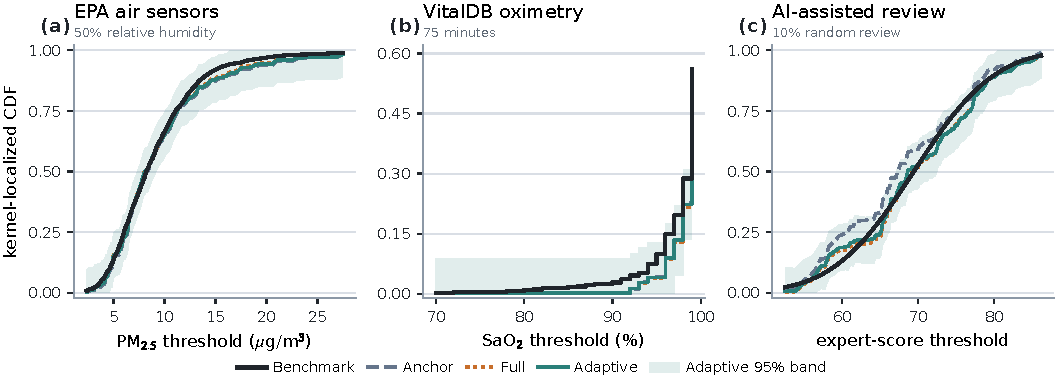
\includegraphics[width=\textwidth]{../paper/figures/figure4_application_evidence.pdf}
\caption{Conditional-CDF estimates from one fixed reference sample in each
study. Each panel uses a 10\% random-reference sample at a target fixed before
the curves were produced. Black denotes \(F_{h,\mathrm{emp}}\) for EPA and
VitalDB and the frozen \(F_{h,0}\) for the AI benchmark; slate dashed, orange
dotted, and teal solid curves denote Anchor, Full, and Adaptive. The teal
ribbon is the Adaptive 95\% simultaneous band. The EPA and AI bands contain
their benchmarks; the VitalDB band does not.}
\label{fig:supp-fixed-application-cdfs}
\end{figure}

\subsection{Oracle mechanisms}

Supplementary Table~\ref{tab:sim-oracle} reports the oracle geometry. The sign
of $2G_h-H_h$ matches the realized anchor-minus-Full ISE direction in all 18
cells. M4 now has separate clipped and raw paths. The clipped paths have
positive transfer signals, while the raw paths have negative signals; both
versions agree with their realized risk directions. M5--M6 have
$\lambda_h^{\mathrm{or}}=0$, mean estimated coefficients below $10^{-4}$, and harmful
full borrowing.

Oracle $m_0(X,S)$ reduces mean ISE relative to the $X$-anchor by 25.3--28.0\%
in M1--M2. In M2, the conservative candidate improves on the anchor but does
not attain the oracle-$m$ risk, illustrating the positive-semidefinite
augmentation excess directly.

\subsection{Candidate regression methods and local failure}

Supplementary Table~\ref{tab:sim-feasible} compares the primary
location--scale learner with misspecified parametric and nearest-neighbor
candidates. At moderate surrogate noise, Adaptive gains are 23.7\%, 25.3\%,
and 22.4\% for the primary, L2, and L3 learners. Across the strong-to-weak
surrogate sequence, primary gains decline from 48.5\% to 7.6\%; the analogous
L2 range is 49.8--11.0\% and the L3 range is 37.0--8.0\%.

The local-reversal scenario N5 is the main failure audit. Adaptive reduces
mean borrowing to 0.0017 and negative-transfer frequency to 1.5\%, compared
with 82.3\% for Full. Its mean ISE remains 0.066\% above the anchor because a
small number of loss realizations dominate the paired mean. This result
shows that Adaptive greatly reduces the risk increase caused by local reversal,
but does not establish uniform or finite-sample dominance.

\subsection{Distributional perturbations and localization dimension}

Adaptive gains are 15.6\%, 17.8\%, and 24.7\% under standardized $t_3$,
standardized $\chi^2_3$, and Gaussian-mixture errors, compared with 22.0\%
under Gaussian errors. For the ten-level outcome, category-scale oracle truth
produces a 22.5\% Adaptive gain and a 25.9\% Full gain. The old apparent loss
was caused by evaluating discrete outcomes against a continuous-scale truth
engine.

With $X=(X_1,X_2)$, a product Epanechnikov kernel, and $h=M^{-1/6}$, Adaptive
gains range from 20.9\% to 24.4\% over
$M\in\{2{,}000,5{,}000\}$ and $p_M\in\{0.10,0.20\}$.

\subsection{Bandwidth, curvature, and estimated propensities}

The bandwidth and denominator-floor checks preserve the primary risk ordering.
The numerical analyses use a denominator floor of $10^{-8}$.
We vary the candidate-path scale over
$s\in\{1,0.5,0.25,0.125,0\}$, so normalized curvature follows $s^2$,
the effective correction decreases from 0.899 to zero, and
Adaptive-minus-path-oracle regret decreases from $6.01\times10^{-5}$ to zero.

Eight exploratory configurations estimate verification probabilities on the
fitting fold. Adaptive gains range from 22.9--45.4\%, while mean borrowing
ranges from 0.408 to 0.600. These results demonstrate sensitivity of the
selected path to propensity estimation; inferential validity still requires
the local product-rate condition in Section~\ref{sec:supp-pi-adaptive}.

\subsection{Scarcity and multiplier bands}

Supplementary Table~\ref{tab:sim-scarcity} reports scaling over four sample
sizes and four reference fractions. For $Mp_Mh\geq30$, scaled ISE lies in
0.319--0.358 for the anchor and 0.241--0.286 for Adaptive. The rescaling is
stable over the grid, while selective placement changes the covariance
constant at the same nominal reference fraction.

Supplementary Table~\ref{tab:sim-bands} reports the 24 multiplier cells.
At the lowest nominal rate index, the selective-verification cells give
Adaptive coverage 0.910--0.935 and anchor coverage 0.908--0.932. The minimum
Adaptive estimate has Monte Carlo standard error 0.0090 and a 95\% Wilson
interval of 0.8907--0.9262. Adaptive coverage over all cells ranges from 0.910
to 0.953. Mean coverage under selective verification increases from 0.9220 at
$p_M=0.05$ to 0.9435 at $p_M=0.20$.
Aligned surrogates reduce
integrated width to 0.760--0.981 of the anchor width; locally reversed paths
produce ratios within 1.000--1.003, eliminating nearly all width gain.
The minimum role-fold verified support averages about five in the lowest
selective cells. Table~\ref{tab:band-local-information} shows pooled raw
coverage of 0.911 for counts 4--5 and 0.945 for counts of at least 10.

A pre-specified seven-cell sensitivity used the same data streams and 4,999
multiplier draws. Increasing rearrangement of the endpoints raised coverage in
several low-information cells but did not restore the nominal level uniformly.
A pointwise-studentized supremum band produced coverage 0.358--0.633 and was
13--24\% narrower than the unstudentized band. It failed the selection rule, so
the raw-process band remains primary.

\subsection{Application configurations}

The EPA analysis uses
\(X=(\mathrm{RH}-50)/20\),
\(S=\log(1+\mathrm{PurpleAir})\), and
\(Y=\log(1+\mathrm{reference\ PM}_{2.5})\). Targets
\(x_0\in\{-1,0,1\}\) correspond to 30\%, 50\%, and 70\% relative humidity;
the Epanechnikov bandwidth is \(h=0.5\), and the 101 thresholds span the
empirical 0.01--0.99 quantiles of transformed \(Y\).

The VitalDB analysis uses
\(X=\log(1+\mathrm{elapsed\ minutes})\), \(S=\mathrm{SpO}_2\), and
\(Y=\mathrm{SaO}_2\). Targets are 30, 75, and 180 minutes, the Epanechnikov
bandwidth is \(h=0.55\), and the threshold grid is \(70{:}99\).

The AI analysis uses standardized complexity \(X\), automated score \(S\),
and the mean of three expert ratings as \(Y\), with \(x_0=0\), \(h=0.3\),
and 101 thresholds defined by point-target conditional quantile levels
0.02--0.98. For confidence-triggered designs, the broadly observed vector is
\(W=(X,S,C)\), where model confidence \(C\) enters the known verification
probability; the augmentation candidates use \((X,S)\). The risk benchmark is
the frozen population \(F_{h,0}\).

\subsection{EPA details}

The EPA source archive is verified by SHA-256 before extraction. The
uncorrected PurpleAir records are aggregated to 2,814 site-days, and calendar
weeks are assigned to regression fitting, weight selection, and CDF evaluation.
At the 10\% random budget, Adaptive gains
are 52.2--60.3\%, with paired intervals excluding zero. A single weekly
cluster-multiplier diagnostic gives 19--30\% narrower Adaptive bands and
complete-data containment at all three humidity targets; it is not a
repeated-coverage result.

\subsection{VitalDB details}

The VitalDB acquisition and hash-selection rules produce 8,476 eligible pairs
and 3,178 subject-level observations. At the 10\% random budget, Adaptive gains
are 11.8\%, 11.2\%, and 2.95\%. Within-grid information multipliers are 1.109,
1.102, and 1.027 at 30, 75, and 180 minutes. Full has lower mean ISE, but its
paired advantage is conclusive only at 30 minutes. Adaptive reduces observed
negative-transfer frequency relative to Full at all targets; the paired
interval excludes zero at 75 and 180 minutes.

\subsection{AI-assisted evaluation details}

The corrected reference uses fixed expert biases $(-1,0,1)$ while retaining
the same dossier text and 5,997 valid model responses. On Corpus A, bias,
MAE, and RMSE are 0.350, 2.415, and 3.058; Pearson and Spearman correlations
are 0.946 and 0.942.

The primary evaluator is \texttt{deepseek-v4-pro};
\texttt{deepseek-v4-flash} is used for the model-sensitivity analysis. Both use
the frozen dossier text and rubric. A canonical call manifest links each
corpus row to its request hash and cached response-file checksum; the model
outputs themselves were fixed before any reference mask was drawn. A companion
cache manifest checksums all retained primary and sensitivity responses.

Under random review, Adaptive gains are 53.9--59.9\%. For fractions up to 0.10,
the anchor needs 2.28--2.50 times the actual fraction to match Adaptive risk
within the evaluated grid. Under local under-review and local reversal,
Adaptive borrowing collapses toward zero and limits mean loss to at most
0.39\%, whereas Full remains harmful. Representative AI multiplier cells have
Adaptive coverage 0.940--0.974 and narrower bands than the anchor.

\subsection{Complete simulation tables}

\begin{table}[p]
\centering
\caption{Oracle mechanism results. The realized gain is anchor ISE minus full-borrowing ISE.}
\label{tab:sim-oracle}
\begin{tabular}{lcccccc}
\toprule
Scenario & $G_h$ & $H_h$ & $2G_h-H_h$ & $\lambda_h^{\mathrm{or}}$ & $E(\widehat\lambda_h)$ & Realized gain \\
\midrule
M1-R1 & 0.575 & 0.575 & 0.575 & 1.000 & 0.900 & 0.001 \\
M1-R2 & 0.861 & 0.861 & 0.861 & 1.000 & 0.852 & 0.001 \\
M2-R1 & 0.287 & 0.144 & 0.431 & 1.000 & 0.998 & 0.001 \\
M2-R2 & 0.431 & 0.215 & 0.646 & 1.000 & 0.984 & 0.001 \\
M3-R1 & 0.750 & 0.998 & 0.501 & 0.751 & 0.734 & 0.001 \\
M3-R2 & 1.131 & 1.515 & 0.746 & 0.746 & 0.721 & 0.001 \\
M4-R1 & 0.867 & 1.445 & 0.290 & 0.600 & 0.595 & 0.001 \\
M4-R1-unclip & 1.437 & 3.593 & -0.719 & 0.400 & 0.399 & -0.001 \\
M4-R2 & 1.321 & 2.239 & 0.403 & 0.590 & 0.582 & 0.001 \\
M4-R2-unclip & 2.153 & 5.381 & -1.076 & 0.400 & 0.391 & -0.002 \\
M5-R1 & -0.269 & 0.130 & -0.667 & 0.000 & 0.000 & -0.001 \\
M5-R2 & -0.404 & 0.196 & -1.005 & 0.000 & 0.000 & -0.002 \\
M6-R1 & -0.269 & 0.130 & -0.667 & 0.000 & 0.000 & -0.001 \\
M6-R2 & -0.404 & 0.196 & -1.005 & 0.000 & 0.000 & -0.002 \\
M7-R1 & 0.507 & 0.532 & 0.481 & 0.952 & 0.873 & 0.001 \\
M7-R2 & 0.733 & 0.779 & 0.687 & 0.941 & 0.837 & 0.001 \\
M8-R1 & 0.567 & 0.687 & 0.448 & 0.826 & 0.794 & 0.001 \\
M8-R2 & 0.836 & 1.025 & 0.646 & 0.815 & 0.742 & 0.001 \\
\bottomrule
\end{tabular}
\end{table}

\begin{table}[p]
\centering
\caption{Feasible estimator results. Relative gain is the percentage reduction in mean ISE from the X-anchor.}
\label{tab:sim-feasible}
\resizebox{\textwidth}{!}{%
\begin{tabular}{lccccccc}
\toprule
Scenario & ISE anchor & ISE Adaptive & ISE Full & Rel. gain & $\widehat\lambda_h$ & NT Adaptive & NT Full \\
\midrule
F1-p0.05 & 0.0099 & 0.0075 & 0.0069 & 23.4 & 0.693 & 0.332 & 0.346 \\
F1-p0.10 & 0.0048 & 0.0036 & 0.0035 & 24.0 & 0.784 & 0.339 & 0.360 \\
F1-p0.20 & 0.0024 & 0.0019 & 0.0018 & 21.5 & 0.850 & 0.362 & 0.383 \\
F2-L2-t16 & 0.0049 & 0.0044 & 0.0043 & 11.0 & 0.699 & 0.388 & 0.419 \\
F2-L2-t4 & 0.0050 & 0.0025 & 0.0023 & 49.8 & 0.833 & 0.219 & 0.223 \\
F2-L2-t8 & 0.0047 & 0.0035 & 0.0034 & 25.3 & 0.781 & 0.349 & 0.353 \\
F2-L3-t16 & 0.0049 & 0.0045 & 0.0044 & 8.0 & 0.730 & 0.381 & 0.396 \\
F2-L3-t4 & 0.0049 & 0.0031 & 0.0030 & 37.0 & 0.947 & 0.207 & 0.213 \\
F2-L3-t8 & 0.0050 & 0.0039 & 0.0038 & 22.4 & 0.880 & 0.313 & 0.319 \\
F2-t16 & 0.0047 & 0.0044 & 0.0043 & 7.6 & 0.683 & 0.429 & 0.443 \\
F2-t4 & 0.0049 & 0.0025 & 0.0023 & 48.5 & 0.835 & 0.203 & 0.222 \\
F2-t8 & 0.0047 & 0.0036 & 0.0035 & 23.7 & 0.787 & 0.337 & 0.370 \\
F3-M1000 & 0.0082 & 0.0066 & 0.0063 & 19.1 & 0.713 & 0.379 & 0.391 \\
F3-M2000 & 0.0049 & 0.0037 & 0.0035 & 24.7 & 0.776 & 0.342 & 0.356 \\
F3-M4000 & 0.0027 & 0.0021 & 0.0020 & 25.3 & 0.835 & 0.350 & 0.361 \\
\bottomrule
\end{tabular}
}
\end{table}

\begin{table}[p]
\centering
\caption{Scarce-reference scaling: ISE times the local-information rate index.}
\label{tab:sim-scarcity}
\begin{tabular}{lccccc}
\toprule
Scenario & $M$ & $p_M$ & $Mp_Mh$ & X-anchor & Adaptive \\
\midrule
SC-M1000-p0.025 & 1000 & 0.025 & 7.5 & 0.341 & 0.325 \\
SC-M1000-p0.050 & 1000 & 0.050 & 15.0 & 0.347 & 0.296 \\
SC-M2000-p0.025 & 2000 & 0.025 & 15.0 & 0.364 & 0.313 \\
SC-M1000-p0.100 & 1000 & 0.100 & 30.0 & 0.344 & 0.286 \\
SC-M2000-p0.050 & 2000 & 0.050 & 30.0 & 0.345 & 0.277 \\
SC-M4000-p0.025 & 4000 & 0.025 & 30.0 & 0.348 & 0.283 \\
SC-M1000-p0.200 & 1000 & 0.200 & 60.0 & 0.337 & 0.267 \\
SC-M2000-p0.100 & 2000 & 0.100 & 60.0 & 0.329 & 0.263 \\
SC-M4000-p0.050 & 4000 & 0.050 & 60.0 & 0.332 & 0.258 \\
SC-M8000-p0.025 & 8000 & 0.025 & 60.0 & 0.338 & 0.263 \\
SC-M2000-p0.200 & 2000 & 0.200 & 120.0 & 0.358 & 0.274 \\
SC-M4000-p0.100 & 4000 & 0.100 & 120.0 & 0.332 & 0.256 \\
SC-M8000-p0.050 & 8000 & 0.050 & 120.0 & 0.340 & 0.261 \\
SC-M4000-p0.200 & 4000 & 0.200 & 240.0 & 0.319 & 0.241 \\
SC-M8000-p0.100 & 8000 & 0.100 & 240.0 & 0.327 & 0.249 \\
SC-M8000-p0.200 & 8000 & 0.200 & 480.0 & 0.323 & 0.250 \\
\bottomrule
\end{tabular}
\end{table}

\begin{table}[p]
\centering
\caption{Raw-process multiplier-band coverage and width (target 0.95). Each cell uses 1,000 replications and 4,999 multiplier draws. Here $M=2{,}000$ and $h=0.30$, so $Mp_Mh=30,60,120$; coverage Monte Carlo standard errors across both methods range from 0.0062 to 0.0091.}
\label{tab:sim-bands}
\begin{tabular}{lllcccc}
\toprule
$p$ & Ver. & Condition & Cov. Adaptive & Cov. anchor & Width Adaptive & Width anchor \\
\midrule
0.05 & R1 & strong & 0.934 & 0.927 & 0.390 & 0.511 \\
0.05 & R1 & moderate & 0.933 & 0.929 & 0.452 & 0.508 \\
0.05 & R1 & weak & 0.928 & 0.935 & 0.496 & 0.511 \\
0.05 & R1 & locally failed & 0.946 & 0.944 & 0.508 & 0.508 \\
0.05 & R2 & strong & 0.935 & 0.932 & 0.518 & 0.644 \\
0.05 & R2 & moderate & 0.910 & 0.908 & 0.582 & 0.633 \\
0.05 & R2 & weak & 0.926 & 0.921 & 0.620 & 0.632 \\
0.05 & R2 & locally failed & 0.917 & 0.919 & 0.643 & 0.641 \\
0.10 & R1 & strong & 0.948 & 0.942 & 0.275 & 0.362 \\
0.10 & R1 & moderate & 0.937 & 0.942 & 0.321 & 0.361 \\
0.10 & R1 & weak & 0.941 & 0.945 & 0.350 & 0.362 \\
0.10 & R1 & locally failed & 0.939 & 0.940 & 0.363 & 0.363 \\
0.10 & R2 & strong & 0.946 & 0.918 & 0.363 & 0.463 \\
0.10 & R2 & moderate & 0.939 & 0.921 & 0.416 & 0.460 \\
0.10 & R2 & weak & 0.946 & 0.939 & 0.444 & 0.456 \\
0.10 & R2 & locally failed & 0.940 & 0.938 & 0.458 & 0.458 \\
0.20 & R1 & strong & 0.945 & 0.932 & 0.201 & 0.256 \\
0.20 & R1 & moderate & 0.940 & 0.945 & 0.230 & 0.257 \\
0.20 & R1 & weak & 0.953 & 0.960 & 0.249 & 0.258 \\
0.20 & R1 & locally failed & 0.948 & 0.948 & 0.257 & 0.257 \\
0.20 & R2 & strong & 0.945 & 0.943 & 0.258 & 0.329 \\
0.20 & R2 & moderate & 0.936 & 0.938 & 0.295 & 0.328 \\
0.20 & R2 & weak & 0.948 & 0.944 & 0.314 & 0.324 \\
0.20 & R2 & locally failed & 0.945 & 0.946 & 0.327 & 0.327 \\
\bottomrule
\end{tabular}
\end{table}

\begin{table}[p]
\centering
\small
\caption{Raw-process coverage by the minimum number of verified kernel-support observations in any role fold, pooled over the 24 band cells.}
\label{tab:band-local-information}
\begin{tabular}{lrrr}
\toprule
Minimum role-fold count & Replications & Adaptive & Anchor \\
\midrule
0--3 & 890 & 0.875 & 0.867 \\
4--5 & 2,378 & 0.911 & 0.912 \\
6--9 & 5,128 & 0.943 & 0.936 \\
10+ & 15,604 & 0.945 & 0.943 \\
\bottomrule
\end{tabular}
\end{table}

\begin{table}[p]
\centering
\small
\caption{Vanishing-path components as the candidate-path scale $s$ approaches zero. The final column is the mean Adaptive-minus-path-oracle ISE gap multiplied by $10^5$.}
\label{tab:sim-vanishing}
\begin{tabular}{@{}rrrrr@{}}
\toprule
$s$ & Relative curvature & $E(\widehat\lambda_h)$ &
$s\,E(\widehat\lambda_h)$ & ISE gap $(\times10^5)$ \\
\midrule
1.000 & 1.0000 & 0.8990 & 0.8990 & 6.010 \\
0.500 & 0.2500 & 0.9986 & 0.4993 & 0.100 \\
0.250 & 0.0625 & 0.9998 & 0.2499 & 0.016 \\
0.125 & 0.0156 & 1.0000 & 0.1250 & 0.000 \\
0.000 & 0.0000 & 0.0000 & 0.0000 & 0.000 \\
\bottomrule
\end{tabular}
\end{table}

\clearpage

\section{Connections to adjacent methods}
\label{sec:comparison}

\begin{table}[H]
\centering
\caption{Comparison with adjacent prediction-assisted, semi-supervised, validation-sample, and local-distribution methods.}
\label{tab:method-comparison}
\scriptsize
\setlength{\tabcolsep}{3.2pt}
\begin{tabular}{>{\raggedright\arraybackslash}p{1.85cm}>{\raggedright\arraybackslash}p{2.05cm}>{\raggedright\arraybackslash}p{1.25cm}>{\raggedright\arraybackslash}p{1.65cm}>{\raggedright\arraybackslash}p{1.25cm}>{\raggedright\arraybackslash}p{1.65cm}>{\raggedright\arraybackslash}p{1.75cm}}
\toprule
Method & Primary target & Fixed continuous $x_0$ & Selective MAR reference sampling & $p_M\to0$ & Entire CDF and simultaneous bands & Transfer or efficiency control\\
\midrule
Validation-sample inference \citep{Pepe1992,TaoZengLin2017}
& Regression parameters under validation or two-phase measurement
& No shrinking point target
& Yes
& Fixed-overlap theory
& No local CDF result
& Likelihood and semiparametric efficiency\\
PPI/PPI++ \citep{AngelopoulosEtAl2023,AngelopoulosDuchiZrnic2023}
& Means and estimating-equation targets
& No
& Labeled and prediction samples
& Not part of the main theory
& Scalar or finite-dimensional inference
& Prediction correction and scalar power tuning\\
Adaptive and safe semi-supervised inference \citep{SongLinZhou2024,DengEtAl2024,ChenEtAl2025}
& Finite-dimensional M-parameters or high-dimensional regression coefficients
& No shrinking point target
& Labeled and unlabeled, or selectively validated, samples
& Not combined with local effective information
& No local CDF process
& Optimal, safe, or regularized auxiliary-information weights\\
PPCI \citep{SuiEtAl2026}
& Conditional functionals at a test point
& Yes
& Labeled and unlabeled samples in the main formulation
& Not part of the main theory
& Pointwise conditional-functional inference
& Prediction-assisted localization and variance reduction\\
PAS \citep{LiIgnatiadis2025}
& A collection of mean-estimation tasks
& No
& Gold-standard outcomes and predictions across tasks
& Not part of the main theory
& No conditional-CDF result
& Empirical-Bayes shrinkage across tasks\\
Decaying-overlap semi-supervised inference \citep{TestaEtAl2025}
& General smooth semiparametric targets
& No shrinking point target
& Yes
& Yes
& Target-specific asymptotic normality
& General influence-function theory under decaying overlap\\
Surrogate-assisted transported distribution inference \citep{Wang2026}
& Transported counterfactual CDFs and quantiles
& No
& Source validation subset and target covariates
& No decaying-validation result
& Uniform transported CDF and quantile bands
& Efficient influence functions for transported distributional targets\\
Local distribution and conditional density \citep{CattaneoJanssonMa2024,CattaneoEtAl2024}
& Conditional distributions and densities
& Yes
& Fully observed outcomes
& Not applicable
& Yes
& Local-polynomial distribution and density estimation\\
Present method
& $F_0(\cdot\mid x_0)$ and its kernel-localized version
& Yes
& Yes
& Yes
& Yes
& Canonical gradient, exact transfer sign, common borrowing weight, and path-oracle equivalence\\
\bottomrule
\end{tabular}
\end{table}

Convolution-smoothed prediction-powered quantile-regression estimators
\citep{TakeishiDingHe2026} target finite-dimensional coefficients with limited
gold-standard outcomes, rather than a local CDF process under selective
verification. The present method estimates a local conditional CDF when the
reference outcome is selectively observed, a surrogate is broadly available,
and the verification fraction may decrease. The canonical gradient gives the
efficiency bound, and the quadratic criterion determines how much surrogate
information to use. Sample splitting separates weight selection from CDF
evaluation. The triangular-array limit then supports simultaneous CDF and
quantile inference.


\bibliographystyle{plainnat}
\bibliography{../paper/references,../paper/references_submission,../paper/references_empirical_process}
\end{document}
